\documentclass[11pt,a4paper]{article}

\usepackage[margin=1.1in]{geometry}
\usepackage{amsmath,amssymb,amsthm,mathtools}
\usepackage[T1]{fontenc}
\usepackage{microtype}
\microtypesetup{expansion=false}
\usepackage{tikz}
\usetikzlibrary{positioning,arrows.meta,calc,fit,backgrounds,patterns}
\usepackage{booktabs,array}
\usepackage{listings}
\usepackage{stmaryrd}
\usepackage[hidelinks]{hyperref}
\usepackage{enumitem}

\theoremstyle{plain}
\newtheorem{theorem}{Theorem}
\newtheorem{proposition}[theorem]{Proposition}
\newtheorem{lemma}[theorem]{Lemma}
\newtheorem{corollary}[theorem]{Corollary}
\newtheorem{conjecture}[theorem]{Conjecture}
\theoremstyle{definition}
\newtheorem{definition}[theorem]{Definition}
\newtheorem{observation}[theorem]{Observation}
\newtheorem{example}[theorem]{Example}
\theoremstyle{remark}
\newtheorem{remark}[theorem]{Remark}

\newcommand{\rhoc}{\textsf{rho}}
\newcommand{\Nil}{\mathbf{0}}
\newcommand{\sepc}{\mathbin{\big|}}
\newcommand{\Hq}{\mathsf{H}}
\newcommand{\out}{\mathsf{out}}
\newcommand{\inn}{\mathsf{in}}
\newcommand{\Rnn}{\mathbb{R}_{\geq 0}}
\newcommand{\Cx}{\mathbb{C}}
\newcommand{\Terms}{\mathcal{T}}
\newcommand{\Cfg}{\mathcal{C}}
\newcommand{\Wt}{\mathcal{W}}
\newcommand{\Red}{\mathrm{Red}}
\newcommand{\prop}{\mathbf{a}}
\newcommand{\wmap}{w}
\newcommand{\dpt}{d}
\newcommand{\gfac}{g}
\newcommand{\funds}{\mathrel{\vdash_{\!\$}}}
\newcommand{\class}{\mathrm{cls}}
\newcommand{\dbr}[1]{\llbracket #1 \rrbracket}

\lstdefinestyle{rho}{
  basicstyle=\ttfamily\footnotesize,
  keywordstyle=\bfseries,
  commentstyle=\itshape,
  morekeywords={new,in,for,contract,match,if,else,true,false,Nil,where,and,or,not,
                exists,forall,nu,rules,rewrites,equations,types,language,name},
  morecomment=[l]{//},
  columns=fullflexible,
  breaklines=true,
  breakatwhitespace=false,
  showstringspaces=false,
  frame=none,
  xleftmargin=1em
}
\lstset{style=rho}

\title{\textbf{Weighted Graph-Structured Lambda Theories}\\[0.4em]
\large Stochastic and quantum execution for MeTTaIL, with a spiking\\
recurrent network as a worked example}
\author{A F1R3FLY.io working note}
\date{August 2026 \\[0.2em]\small Second version, revised in response to referee comments}

\begin{document}
\maketitle

\begin{abstract}
We equip the rewrite rules of a finitely presentable graph-structured lambda theory (GSLT), as
presented in MeTTaIL, with \emph{weight maps}: finite maps whose keys are spatial--behavioural
formulae refining the left-hand side of a rule and whose values are weights. A weight map instance
is part of a state specification, so a rewrite may update it; weights are therefore dynamic. We
develop the construction in three movements. First, we impose a \emph{partition discipline} on the
key set --- the refinements of a rule's left-hand side must be pairwise exclusive and jointly
exhaustive --- and show that this single requirement is what makes the weighting a total,
single-valued classification of redexes; we then say what it costs, which is a dilemma rather than a
theorem: a partition stated inside the generated logic demands Boolean structure of the target
specification, and a partition stated outside it forfeits specification closure. Second, with
weights in $\Rnn$ we define propensity as $\prop = \wmap(\varphi)\cdot\sum_k \gfac(k)$ over
classified, funded redex positions and obtain a Gillespie simulator; we prove that the construction
restricted to the summation-free $\pi$-calculus, static maps, and channel-identity keys is exactly
the Stochastic Pi Machine, and that dynamic maps take it strictly beyond. Third, with weights in
$\Cx$ we use the complex coalgebra coefficients directly as amplitudes of a linear transition
operator on the Hilbert space spanned by reachable \emph{configurations}, terms paired with weight
maps. A single global normalisation makes that operator a contraction $T$ without changing its
relative phases or its normalised postselected output. The Julia--Halmos defect construction embeds
$T$ in a unitary on the system and one auxiliary qubit: the zero branch applies $T$ and the one branch
records failure. Repeating the construction with $n$ fresh auxiliaries and postselecting their
all-zero state implements $T^n$. Absolute squares enter only when those auxiliaries or the system are
measured, so interference occurs in the rewrite amplitudes themselves; structural equations remain
quotient identifications and no separate Hamiltonian is introduced. The
worked example is an asynchronous stochastic spiking recurrent network in a weighted \rhoc\ theory:
neurons are persistent for-comprehensions, synaptic efficacies live in the weight map rather than in
the payload, thresholds are join structure, a saturating response emerges from the chain rather than
being written into a term, and a minimal local Hebbian potentiation rule is exactly the refinement
entries' update functions --- so that learning and inference are the same transition relation,
differing only in which component of the state they touch.
\end{abstract}

\tableofcontents

\section{Introduction}
\label{sec:intro}

A rewrite rule's left-hand side is a type. Terms inhabit it; the rule fires at its inhabitants. This
note is about what happens when one refines that type and attaches a number to each refinement.

The move is small to state and consequential to develop. A GSLT is a triple $(\Sigma, E, R)$: a
signature which is in general a lambda theory, a set of equations imposing a structural congruence,
and an adjoined graph of rewrite rules \cite{omnibus}. Given such a presentation, the OSLF family of
algorithms generates a logic from it, with one structural connective per term former of $\Sigma$ and
one context-labelled modality per rule of $R$ together with a choice of redex position
\cite{omnibus,classifier}. The formulae of that generated logic are exactly the vocabulary in which
one can refine a rule's left-hand side --- and they are generated, not designed, so the refinements
come for free with the theory. To weight a rule is to give a finite map
\[
\varphi_1 \mapsto v_1, \quad \ldots, \quad \varphi_m \mapsto v_m
\]
from such refinements to weights. A term's redexes are then classified by which refinement they
satisfy. Real weights turn the enabled redexes into a rate distribution; complex weights turn the
same classified transition graph into a linear amplitude operator.

Two things distinguish this from the existing literature on stochastic process calculi.

\paragraph{Keys are formulae, not names.} In Priami's stochastic $\pi$-calculus \cite{priami} and in
Phillips and Cardelli's Stochastic Pi Machine (SPiM) \cite{spim,spim-sim}, a rate is attached to a
\emph{channel}. That is one refinement among many: ``this redex is a communication on $n$'' is a
particular formula in the generated logic, and there is no reason the modeller should be restricted
to it. Once keys are formulae, a rate may depend on the shape of the payload, on the \emph{namespace}
a channel belongs to --- which in a reflective calculus is real structure, reachable by the classifier
through the name predicate $@\varphi$, and is what lets one key cover a growing population of
channels (\S\ref{sec:rnn-uniform}) --- or on any Boolean combination of these. Channel identity is
recovered as the degenerate case (\S\ref{sec:spim}). We are careful not to claim more than that. The
classifier of Proposition~\ref{prop:classify} evaluates its formula at the matched left-hand side
$L\sigma$ and not at $k[L\sigma]$, so the ambient context is not visible to a key at all; properties
of a redex's \emph{position} are the business of the geometric factor $\gfac(k)$ (\S\ref{sec:geometric}),
and the division of labour between the two is clean only because it is respected.

\paragraph{Maps are state, not declaration.} A weight map instance is part of a state
specification. A rule's refinement entries therefore carry not only a weight but an \emph{update
function} on the whole map, applied when the rule fires. Rates change during execution. SPiM does
not permit this --- its rates are fixed at declaration --- and the restriction is not incidental to
its design but constitutive of it, since a static rate function is what makes the underlying object
a time-homogeneous CTMC over terms alone. We recover Markovianity by a different route: the weight
map is \emph{in} the state, so the chain is over configurations $(P, \wmap)$ rather than over terms
(\S\ref{sec:gillespie}). This is the technical content of ``the map may be updated,'' and it is what
the worked example of \S\ref{sec:rnn} needs, because plasticity is nothing other than a weight-map
update.

Two further points of scope. The construction is generic over the GSLT: it applies to any theory
one can write down in MeTTaIL's \texttt{language!} block \cite{mettail}, so one obtains a stochastic
machine for the ambient calculus, for a user-defined DSL, or for the \rhoc\ calculus, by writing the
theory rather than by writing a simulator. And the weight codomain selects an execution. We treat two
instances: $\Rnn$, giving classical Gillespie simulation (\S\ref{sec:gillespie}); and $\Cx$, giving
a complex transition operator together with a postselected unitary dilation
(\S\ref{sec:quantum}). The two instances share classification and the weighted transition graph but
not a propensity interpretation. A third instance --- weights in a quantale, giving a fuzzy calculus
--- is deliberately out of scope here; see \cite{fuzzy}.

\paragraph{What is new.} Beyond the two distinguishing points above:
\begin{enumerate}[label=(\roman*),leftmargin=2.2em]
\item The \emph{partition discipline} of \S\ref{sec:refinement}, and the observation that it is not
a technicality but the condition under which weighting is well defined at all --- together with an
account of what it costs, namely that stating it internally demands Boolean structure of the target
logic specification while stating it externally forfeits specification closure
(\S\ref{sec:boolean}).
\item A propensity formula (\S\ref{sec:propensity}) that separates four factors which the literature
usually conflates: the refinement's weight, a geometric factor accumulated up the context rules,
redex multiplicity, and a funding gate supplied by cost accounting.
\item Theorem~\ref{thm:spim}: the summation-free fragment of SPiM is the construction's restriction,
exactly.
\item Definition~\ref{def:transition-operator}, which uses the complex weights before any Born rule:
derivations with a common target add as amplitudes in one matrix element, so their relative phases
can reinforce or cancel.
\item The unitary defect dilation of Theorem~\ref{thm:unitary-dilation} and the all-zero branch theorem
(Theorem~\ref{thm:postselected-power}), which implement $T$ with one auxiliary qubit and $T^n$ with
$n$ fresh auxiliaries.
\item The observation (\S\ref{sec:quantum-logic}) that the OSLF-generated formulae give canonical
basis-diagonal projective measurements of the postselected state.
\item The spiking-network example of \S\ref{sec:rnn}, whose thesis is that \emph{synaptic efficacy is
represented as transition intensity in the operational semantics, and the same transition updates
that intensity}: the efficacies live in the weight map, the threshold lives in the join structure of
a for-comprehension, a saturating response is emergent, and learning is a weight-map update
performed by the same rewrite that performs inference.
\end{enumerate}

\paragraph{Where this note sits.} It supplies the construction that \cite{scientist} cites as
\emph{Stochastic simulation for decorated ciGSLTs} and fills the placeholder section of
\cite{mettacalc}. It depends on \cite{omnibus} for GSLTs and OSLF, on \cite{classifier} and
\cite{scientist} for the shape of the generated spatial--behavioural logic --- which is spelled out
in those papers and not yet present in the implementation branch --- and on \cite{costmonad} for
cost accounting, which enters only in \S\ref{sec:cost} and only as a gate.

\paragraph{Revision note.} This is the second version of this note. The first was read by an external
referee, and most of what follows is a response to that reading. Where a claim has been withdrawn or
weakened we say so at the point of change rather than silently, since a reader of the first version
deserves to be told which of its statements not to rely on. The quantum construction is now built
over a basis of configurations and uses complex weights directly as entries of a transition
operator. The former magnitude-square interpretation, Lindblad jump construction, and Hamiltonian on
un-quotiented structural equations have been removed; they discarded the phases before the rewrite
dynamics and treated representatives of one structural class as distinct states. The replacement
normalises the assembled operator globally, dilates it unitarily by its defects, and obtains powers by
all-zero postselection (\S\ref{sec:quantum}). The other substantive changes remain: the necessity
claim about Boolean target specifications is weakened and replaced by a dilemma
(\S\ref{sec:boolean}); the locality lemma is restated for the fragment in which it is true, with a
matching requirement added to admissibility (\S\ref{sec:locality}); the emergent neural response is
exponential-saturating and not logistic (\S\ref{sec:squash}); the SPiM theorem is titled for the
fragment it actually proves (\S\ref{sec:spim}); the CTMC generator's diagonal is corrected for
self-transitions (Remark~\ref{rem:selfloop}); and \S\ref{sec:impl} is rewritten against the
implementation that exists rather than against the prototype it superseded.

\section{Background, compressed}
\label{sec:background}

We recall only what the construction uses, and forward everything else to \cite{omnibus}.

\subsection{GSLTs and their presentations}

A \emph{graph-structured lambda theory} is a triple $(\Sigma, E, R)$. The signature $\Sigma$ is a
lambda theory --- terms may contain variables, and binding is part of the presentation, which is
what distinguishes the setting from graph-enriched Lawvere theories. $E$ is a set of equations
imposing a structural congruence $\equiv$ on terms. $R$ is a graph of rewrite rules adjoined to the
structure as a Lawvere theory of graphs, with source and target maps satisfying the minimal
requisite equations. The adjective \emph{graph-structured} captures the rewrites; \emph{lambda
theory} captures term languages with variables.

Rules come in two kinds, and the distinction is load-bearing throughout this note.

\begin{definition}[Base and context rules]
\label{def:rules}
A \emph{base rule} is hypothesis-free:
\[
r \,.\; \vdash\; L \;\leadsto\; R,
\]
with $L, R$ terms of some sort $\tau$ over $\Sigma$, possibly with pattern variables. A
\emph{context rule} is conditional on a rewrite:
\[
c \,.\; \mid S \leadsto T \;\vdash\; C[S] \;\leadsto\; C[T],
\]
for a one-hole context former $C$. Base rules are the ground of the dynamics; context rules are
\emph{addressing} --- they say where a base rule may fire, not that anything happens.
\end{definition}

This is MeTTaIL's actual surface syntax for its \texttt{rewrites} block \cite{mettail}. In the
\rhoc\ presentation, \texttt{Exec} and the communication rule are base; \texttt{ParCong} and
\texttt{NewCong} are context rules.

An \emph{interactive} GSLT is one whose base rules' left-hand sides are headed by a distinguished
family of formers $K$ --- the interaction cut --- across which program and environment meet:
application for the lambda calculus, parallel composition for CCS, $\pi$ and \rhoc. A
\emph{continued} interactive GSLT (ciGSLT) additionally has surfaces and continuations. Everything
below is stated for ciGSLTs, though only the interactive structure is used.

\subsection{Locations}

Write $\partial \Terms$ for the space of one-hole contexts, in the McBride-derivative sense: a
location is a pair $(\partial T, T)$ of a context and the term type. We use $\partial \Terms$ as a
single object playing three roles, as in \cite{omnibus}: the index set of the generated modalities,
the labels on the transition system, and the positions inside a term. It is this identification that
lets a weight be attached to a \emph{position} and read as a modality.

\begin{definition}[Redex]
\label{def:redex}
Let $r \,.\; \vdash L \leadsto R$ be a base rule and $P$ a term. A \emph{redex of $r$ in $P$} is a
\emph{selection} of a one-hole context $k \in \partial\Terms$ and a substitution $\sigma$ for the
pattern variables of $L$ from the decomposition of $P$, such that $P \equiv k[L\sigma]$. Two redexes
are identified when they select the same occurrences; interchanging two occurrences of
$\equiv$-equal subterms yields \emph{distinct} redexes, which happen to have $\equiv$-equal
contracta. Write $\Red_r(P)$ for the set of redexes of $r$ in $P$, and
$\Red(P) = \coprod_r \Red_r(P)$.
\end{definition}

$\Red_r(P)$ is finite for finite $P$ and finitely many rules. The convention on identification is
Gillespie's, and it is the one that matters: two molecules of the same species offer two ways for a
reaction to occur, not one, and a stochastic simulator that identifies them runs at half speed. In
an associative--commutative setting the reactants are drawn from a multiset, so $|\Red_r(P)|$ is a
count of selections from a bag --- $\mathrm{In}\cdot\mathrm{Out}$ for a binary interaction drawing
one reactant from each of two species, $\binom{n}{2}$ for one drawing two from the same species.
Structural congruence is used to \emph{find} the decompositions, not to collapse them.
Remark~\ref{rem:distinct-contracta} records what happens when distinct redexes do share a contractum.

\subsection{The generated logic}
\label{sec:logic}

The following is generated by OSLF from the presentation and is not ours to design. We state it for
the \rhoc\ calculus --- term formers $\Nil$, $*n$, $n!(Q)$, $\texttt{for}(x \leftarrow n)P$,
parallel composition, and $@P$, with parallel composition associative--commutative and a single
communication rewrite --- and note that everything transfers verbatim to any other presentation,
with the connective list changing to match the formers. The presentation follows
\cite[\S2]{classifier} and \cite[\S3]{scientist}; it is not present in the implementation branch,
whose logic is still under development.

\paragraph{Structural connectives.} One connective per term former. $\out(n)\varphi$ holds of
$n!(Q)$ with $Q \models \varphi$; $\inn(n)\varphi$ is the analogue on receipts. Because parallel
composition is associative--commutative, the generated connective for it is a separating
conjunction:
\[
P \models \varphi \sepc \psi
\iff
P \equiv Q \sepc R \text{ with } Q \models \varphi,\ R \models \psi .
\]

\paragraph{Behavioural modalities.} One primitive modality $\langle K_j \rangle$ per rewrite rule
\emph{and choice of redex position}, labelled by the one-hole context in which the step fires. The
index is not decoration. For \rhoc, with a single interaction rule, all the information in a label
is in the position: for $P \equiv K_j[\,\texttt{for}(x \leftarrow n)Q \sepc n!(Q')\,]$ the label
$K_j$ is everything else. Thus $\exists j.\,\langle K_j\rangle\varphi$ and
$\forall j.\,[K_j]\varphi$ quantify over redex positions, and a bare $\langle K \rangle$ abbreviates
the existential.

\paragraph{Name predicates.} A name is a quoted process, so
\[
n \models @\varphi \iff n = @P \text{ with } P \models \varphi ,
\]
which is namespace logic \cite{namespace}: a namespace is described by a property rather than
enumerated. This matters in \S\ref{sec:rnn}, where synapses are picked out by structured names.

\paragraph{Propositional layer.} Conjunction and $\top$ come from the finite-limits fragment;
disjunction, implication and negation require more, and a target specification supplies them or does
not \cite{omnibus}. \S\ref{sec:boolean} shows that weighting \emph{forces} the choice.

\paragraph{Additions.} A greatest fixed point $\nu X.\varphi$ with $X$ positive; the hidden-name
quantifier $\Hq x.\varphi$; graded separation $\varphi \sepc_k \psi$ \cite[\S2.3]{classifier}. We
use $\nu$ only in \S\ref{sec:rnn-uniform}.

\begin{definition}[Depth]
\label{def:depth}
The depth $\dpt(\varphi)$ of a structural formula is the maximal nesting of term-former connectives
and prefixes: $\dpt(\top) = 0$, $\dpt(\out(n)\varphi) = \dpt(\inn(n)\varphi) = 1 + \dpt(\varphi)$,
$\dpt(\varphi \sepc \psi) = \max(\dpt(\varphi), \dpt(\psi))$, $\dpt(@\varphi) = \dpt(\varphi)$,
$\dpt(\Hq x.\varphi) = 1 + \dpt(\varphi)$.
\end{definition}

\subsection{Ideal logic, checkable fragment}

One methodological commitment governs \S\ref{sec:refinement}. Following \cite[\S1.3]{classifier}, we
distinguish the \emph{ideal} logic, adequate for the idealised calculus and the thing that
\emph{defines} a semantic notion, from \emph{fragments}, restricted so that model checking
terminates, which \emph{decide} it. A logic whose model checking terminates is necessarily not
adequate for the whole of a Turing-complete host. The relevance here is sharp and appears at
Requirement~\ref{req:dec}: a simulator evaluates its key formulae at every step, so keys must come
from a checkable fragment. What is elsewhere a methodological trade-off is here an executability
constraint.

\section{Refining a left-hand side}
\label{sec:refinement}

\subsection{The keys}

Fix a base rule $r \,.\; \vdash L \leadsto R$ with $L$ of sort $\tau$. The set of redexes of $r$ is
carved out by the shape of $L$; we want to subdivide it. Write $L^\sharp$ for the structural formula
that characterises the left-hand side pattern --- for the \rhoc\ communication rule,
$L^\sharp = \inn(n)\top \sepc \out(n)\top$ with $n$ existentially bound. The candidate keys are the
formulae of the generated logic that \emph{refine} $L^\sharp$.

\begin{definition}[Refinement]
\label{def:refinement}
A formula $\varphi$ \emph{refines} $L^\sharp$, written $\varphi \sqsubseteq L^\sharp$, when
$\models \varphi \Rightarrow L^\sharp$. The refinements of $L^\sharp$, ordered by entailment, form
the \emph{refinement lattice} $\mathcal{R}(r)$ of the rule.
\end{definition}

We now impose three requirements on a key set $\Phi_r \subseteq \mathcal{R}(r)$. The first is the
substantial one.

\begin{definition}[Partition discipline]
\label{def:partition}
$\Phi_r = \{\varphi_1, \ldots, \varphi_m\}$ is a \emph{partition of $r$} when
\begin{enumerate}[label=(P\arabic*),leftmargin=3em]
\item \emph{Exclusivity}: $\models \neg(\varphi_i \wedge \varphi_j)$ for all $i \neq j$;
\item \emph{Exhaustiveness}: $\models L^\sharp \Rightarrow \bigvee_{i} \varphi_i$.
\end{enumerate}
\end{definition}

\begin{definition}[Requirements on a key set]
\label{def:reqs}
A key set is \emph{admissible} when it is a partition and, in addition:
\begin{enumerate}[label=(R\arabic*),leftmargin=3em]
\item\label{req:dec} \emph{Decidability}: each $\varphi_i$ lies in a fragment for which model
checking terminates on the terms of interest.
\item\label{req:loc} \emph{Locality}: $\dpt(\varphi_i) \le \alpha_r < \infty$ for all $i$, for some
bound $\alpha_r$ fixed with the rule.
\item\label{req:str} \emph{Structurality}: each $\varphi_i$ lies in the structural fragment ---
$\out$, $\inn$, $@$, $\sepc$, ground predicates and the propositional connectives --- carrying no
behavioural modality $\langle K_j\rangle$, no fixed point $\nu X.\varphi$ and no hidden-name
quantifier.
\end{enumerate}
\end{definition}

\ref{req:dec} is forced by execution: a simulator must classify every enabled redex before it can
sample, so a key whose evaluation may diverge is a key that stops the simulation. \ref{req:loc} and
\ref{req:str} are forced by \emph{efficient} execution and pay off together in
Lemma~\ref{lem:locality}. \ref{req:str} is new in this version, and it is a restriction on
\emph{keys} alone: the behavioural modalities and the fixed point remain available for stating and
checking properties of the resulting chain, and \S\ref{sec:rnn-uniform} uses $\nu$ for exactly that.
What they may not do is determine a rate. A rate that depends on what a redex can do next cannot be
recomputed locally when something elsewhere in the term changes, and the incremental scheme of
\S\ref{sec:incremental} is the thing that would break.

\subsection{What the partition buys}
\label{sec:what-partition-buys}

\begin{proposition}[Classification]
\label{prop:classify}
Let $\Phi_r$ be a partition of $r$. Then the assignment
\[
\class_r : \Red_r(P) \longrightarrow \Phi_r,
\qquad
\class_r(k, \sigma) = \text{the unique } \varphi_i \text{ with } L\sigma \models \varphi_i
\]
is a total function, for every term $P$.
\end{proposition}

\begin{proof}
$(k,\sigma) \in \Red_r(P)$ gives $P \equiv k[L\sigma]$, so $L\sigma \models L^\sharp$ by
construction of $L^\sharp$. Exhaustiveness gives $L\sigma \models \varphi_i$ for some $i$, which is
totality; exclusivity gives at most one such $i$, which is single-valuedness. Well-definedness on
$\equiv$-classes holds because satisfaction is $\equiv$-invariant, the generated connectives being
generated from $\Sigma$ modulo $E$.
\end{proof}

This is exactly what fails without the discipline, and it fails in two directions. Without
exhaustiveness the weighting is partial: some enabled redexes have no rate, and one must invent a
convention (fire them at rate zero? at a default rate? refuse to run?) that is not part of the
specification. Without exclusivity the weighting is multi-valued, and one must invent an
\emph{aggregation} (take the most specific key, if a unique minimum exists; sum the weights of all
satisfied keys; take the maximum). Each convention is defensible and each yields a different
simulator from the same specification, which is precisely the situation a specification exists to
prevent.

\begin{remark}[Completing a partition is cheap]
\label{rem:default}
The discipline is less onerous than it looks. Given any pairwise-exclusive family
$\{\varphi_1,\dots,\varphi_m\}$, the family
$\{\varphi_1,\dots,\varphi_m,\ \varphi_\bot\}$ with
$\varphi_\bot := L^\sharp \wedge \neg\bigvee_i \varphi_i$ is a partition, and a modeller who wants
the unlisted redexes inert simply sets $\wmap(\varphi_\bot) = 0$. Exclusivity is the real
constraint; exhaustiveness is a completion. In practice, keys of the form ``the redex is a
communication on channel $n$,'' indexed by distinct $n$, are exclusive for free.
\end{remark}

\subsection{What stating the partition costs}
\label{sec:boolean}

\begin{proposition}[Boolean demand, for an internal statement]
\label{prop:boolean}
Suppose the partition conditions (P1) and (P2) are to be stated \emph{in the generated logic itself},
as Definition~\ref{def:partition} writes them. Then that logic must carry negation, conjunction and
disjunction, and a target logic specification supplying only the finite-limits fragment will not do.
\end{proposition}

\begin{proof}
Immediate from the shape of (P1) and (P2): (P1) mentions $\neg$ and $\wedge$, (P2) mentions
$\Rightarrow$ and $\bigvee$. Finite limits supply $\wedge$ and $\top$ only \cite{omnibus}.
\end{proof}

The hypothesis is doing all the work, and the first version of this note dropped it, concluding
instead that \emph{one cannot weight a theory whose generated logic is too weak to be adequate for
it}. That does not follow. A key family drawn from a positive fragment may perfectly well be
pairwise disjoint and jointly exhaustive; what a weak logic prevents is not the \emph{holding} of
(P1) and (P2) but their \emph{expression} as entailments between formulae of the language the keys
are written in. Exclusivity and exhaustiveness can instead be discharged in the metatheory --- by an
elaborator that checks them on the instances that arise, or by a proof about a schema of keys --- and
the weighting is then perfectly well defined. The choice is a genuine one, and both branches cost
something.

\begin{observation}[The cost of an external partition]
\label{obs:closure}
If (P1) and (P2) are discharged in the metatheory rather than in the generated logic, the
specification is no longer \emph{closed}: whether a key set is admissible becomes a judgment the
object language cannot express, so two implementations conforming to the same written specification
may disagree about admissibility, hence --- by Proposition~\ref{prop:classify} --- about the
classification, hence about the sampled distribution. That is precisely the failure the partition
discipline was introduced to prevent (\S\ref{sec:what-partition-buys}), relocated one level up
rather than removed.
\end{observation}

So a weighted GSLT must choose between a Boolean target specification and an external admissibility
judgment, and it should say which. Our own implementation takes the second branch and pays the stated
price: its partition check is a procedure over witnesses, sound as a refuter and silent as a proof
(\S\ref{sec:built}).

On the first branch there is still a convergence worth recording. The omnibus identifies possession
of something like a negation and a conjunction as exactly the condition under which a generated logic
enjoys an adequacy theorem, and notes that Hypercube-style members of the OSLF family, which generate
type systems, offer no such thing \cite{omnibus}. Proposition~\ref{prop:boolean} says that an
internal statement of the partition makes the same demand for an independent reason. A weighting is a
claim about which behaviours are distinguishable enough to be priced differently, and if that claim
is to be made inside the generated logic it needs the expressive power of the claim that they are
distinguishable at all.

Requirement \ref{req:dec} then pulls the other way, since a terminating fragment is necessarily
inadequate for a Turing-complete host. The two are not in conflict, because they apply to different
artifacts: adequacy is a property of the ideal logic in which the specification is \emph{stated},
and termination is a property of the fragment in which the keys are \emph{evaluated}. A modeller
writes a partition in the ideal logic, then checks that the particular keys chosen happen to lie in
a checkable fragment. \S\ref{sec:rnn} exhibits keys of depth $2$, for which the check is trivial.

\subsection{Locality}
\label{sec:locality}

Lemma~\ref{lem:locality} below is what licenses an incremental simulator. It is true of the
structural fragment and false of the generated logic as a whole, and the first version of this note
stated it for the whole. The counterexamples are not exotic: a behavioural modality
$\langle K_j\rangle\varphi$ inspects the successors of a term rather than a bounded syntactic
neighbourhood of a position, and a greatest fixed point may be refuted only by unbounded inspection,
so neither is confined by a depth bound in the sense Definition~\ref{def:depth} measures.
\ref{req:str} is what restricts the lemma to the fragment where it holds.

A second correction concerns the measure. ``Distance in the term tree'' is not well defined modulo an
associative--commutative equation, since a parallel composition is a multiset and has no canonical
tree; a lemma whose radius depends on a choice of tree is a lemma about a presentation. We use
instead the \emph{component distance} $\delta(k,k')$ between two positions: the number of term-former
occurrences on the shortest path joining them in a decomposition witnessing both, counting one
parallel composition as a single former whatever its arity. $\delta$ is $\equiv$-invariant, because
the decompositions it quantifies over are exactly those the generated connectives quantify over, and
it agrees with tree distance in a presentation with no AC formers.

\begin{lemma}[Locality of reclassification, structural fragment]
\label{lem:locality}
Let all keys of all rules satisfy \ref{req:loc} and \ref{req:str}, with depth at most $\alpha$. Let
$P \equiv k[L\sigma]$ and let $P' \equiv k[R\sigma]$ result from firing that redex. Then for any
redex $(k', \sigma')$ of any rule surviving in $P'$ with
$\delta(k,k') > \alpha + |L| + |R|$, the class $\class(k',\sigma')$ is unchanged.
\end{lemma}

\begin{proof}
By induction on a structural formula $\varphi$ with $\dpt(\varphi) \le \alpha$, satisfaction of
$\varphi$ at a position is determined by the components within $\alpha$ nested formers of it:
$\out$, $\inn$ and $@$ descend one former; $\wedge$, $\vee$ and $\neg$ descend none; and the
separating conjunction quantifies over decompositions of the subterm at that position rather than of
the whole, so it stays inside the same neighbourhood. No case appeals to a rewrite or to an unbounded
unfolding, which is where \ref{req:str} is used and where the lemma would fail without it. The
rewrite replaces $L\sigma$ by $R\sigma$ and leaves $k$ pointwise fixed, so a neighbourhood of radius
$\alpha$ disjoint from the replaced material sees an identical multiset of components; the offset
$|L| + |R|$ accounts for neighbourhoods overlapping the replaced region.
\end{proof}

The point is algorithmic. Recomputing $\class$ over the whole term at every step makes the simulator
quadratic in term size; Lemma~\ref{lem:locality} licenses an incremental propensity update in the
style of Gibson and Bruck's next-reaction method \cite{gibson-bruck}, touching only a bounded
neighbourhood of the fired redex. This is where \ref{req:loc} and \ref{req:str} earn their place, and
it is the reason to prefer shallow structural keys where the modelling permits. A modeller who wants
a modal key is not forbidden one --- the logic is restricted for keying, not for checking --- but the
incremental scheme is then unavailable and the simulator must reclassify globally, which is what our
implementation does and what \S\ref{sec:built} records.

\section{Weighted rewrite systems}
\label{sec:weighted}

\subsection{The weight codomain}

\begin{remark}[Two codomains, two operational meanings]
\label{rem:codomain}
Weights are drawn from a commutative semiring $\mathcal{K}$, and we treat two instances,
\[
\mathcal{K}=\Rnn=(\Rnn,+,\cdot,0,1)
\qquad\text{and}\qquad
\mathcal{K}=\Cx.
\]
They share the key sets, classification, updates, and weighted transition graph, but not the final
interpretation of a coefficient. In $\Rnn$ a weight is a rate, with units of inverse time, and
Definition~\ref{def:propensity} assembles those rates for Gillespie simulation. In $\Cx$ a weight is
an amplitude. It is inserted directly into the matrix element of
Definition~\ref{def:transition-operator}; there is no map $z\mapsto |z|^2$ before that operator is
formed. Magnitude squares appear only as Born probabilities after the operator has been embedded in a
unitary and an auxiliary qubit has been measured. Thus the complex instance retains phase at the
point where different derivations are added.
\end{remark}

\begin{remark}[Rates and global contraction normalisation]
\label{rem:rnn}
We take the real codomain to be $\Rnn$ rather than the unit interval. A real weight is a rate and
there is nothing to normalise it against. The unit interval is available as a derived presentation:
fixing a global clock rate $\Lambda\geq\prop_0$ and setting $p_i=\prop_i/\Lambda$ gives the
uniformised discrete-time chain. Uniformisation is a useful implementation strategy and a poor local
specification, because dynamic maps make the required global bound a reachability obligation.

The complex construction likewise imposes no entrywise bound such as $|z|\leq 1$. Contractivity is a
property of the assembled matrix, not of each weight separately: coherent sums can make an operator
large even when every entry of the map lies in the unit disk. Definition~\ref{def:transition-operator}
therefore forms the full amplitude operator $T_0$ and divides once by
$\alpha=\max\{1,\|T_0\|\}$. This preserves every relative phase and changes only the success
probability of the postselection, not its normalised conditional output.
\end{remark}

\subsection{Weight maps and augmented rules}

\begin{definition}[Weight map]
\label{def:wmap}
Let $(\Sigma, E, R)$ be a GSLT with admissible key sets $\Phi_r$ for each base rule $r$. A
\emph{weight map} is a function
\[
\wmap : \textstyle\coprod_{r} \Phi_r \longrightarrow \mathcal{K}.
\]
Write $\Wt$ for the set of weight maps. Since each $\Phi_r$ is finite and there are finitely many
rules, $\Wt \cong \mathcal{K}^N$ for a fixed $N$.
\end{definition}

\begin{definition}[Configuration]
\label{def:config}
A \emph{configuration} is a pair $\mathfrak{c} = (P, \wmap)$ with $P$ a term modulo $\equiv$ and
$\wmap \in \Wt$. Write $\Cfg$ for the set of configurations.
\end{definition}

The phrase ``a map instance is part of a state specification'' is Definition~\ref{def:config}, and
everything downstream turns on it.

\begin{definition}[Augmented rules]
\label{def:augmented}
An \emph{augmented base rule} is
\[
r \,.\; \vdash\; L \leadsto R \;\; [\,\wmap_r\,]
\;\{\; \varphi_1 \Rightarrow (v_1, u_1), \;\ldots,\; \varphi_m \Rightarrow (v_m, u_m) \;\}
\]
where $\{\varphi_i\}$ is an admissible key set for $r$, $v_i \in \mathcal{K}$ are the initial
weights, and $u_i : \Wt \to \Wt$ are \emph{update functions} on the whole map. An \emph{augmented
context rule} is
\[
c \,.\; \mid S \leadsto T \;\vdash\; C[S] \leadsto C[T] \;\; [\,\gfac_c\,] \;\{\; f_c \;\}
\]
with $\gfac_c \in \Rnn$ a \emph{geometric factor} and $f_c : \Wt^* \times \Wt \to \Wt$ a
\emph{fold function}.
\end{definition}

The initial weight map is $\wmap_0(\varphi_i) = v_i$; the leading $[\wmap_r]$ is a per-rule scalar,
convenient in practice and formally absorbable into the $v_i$, which is how we treat it below.

\subsection{Why context rules carry a factor and not a propensity}
\label{sec:geometric}

The design decision that most distinguishes Definition~\ref{def:augmented} from the obvious
alternative is that context rules do not have propensities of their own.

The obvious alternative gives every rule, base and context alike, a weight and lets the simulator
select among all of them. It double-counts. A step of the transition system is a base rule firing
\emph{somewhere}; the context rules composing the path from the root to that somewhere are the
address of the firing, not additional events. In the vocabulary of the energetics reading of
OSLF-decorated GSLTs, structural rules are addressing, not dynamics, and incur no primitive cost.
Selecting a context rule and then a base rule as though they were independent draws makes a single
event into two.

So context rules contribute multiplicatively, to the propensity of the base firing they address:

\begin{definition}[Geometric factor]
\label{def:gfac}
Let $k \in \partial\Terms$ be a position, obtained by composing context rules $c_1, \ldots, c_p$
from the root inwards. Its \emph{geometric factor} is
$\gfac(k) = \prod_{q=1}^{p} \gfac_{c_q} \in \Rnn$.
\end{definition}

Setting every $\gfac_c = 1$ recovers ``addressing is free'' exactly, and is the default we recommend.
The reason to permit $\gfac_c \neq 1$ is that it is the natural home for a \emph{spatial} bias:
$\gfac$ is a weighting on the reduction graph's edges that depends only on where in the term the
interaction surfaces are, as against $\wmap(\varphi)$, which depends on what is being transferred.
This is the geometric-versus-matter split of the gravitation correspondence \cite{costspacetime}
appearing here as an implementation detail, and we flag it as such without pursuing it.

\subsection{Dynamics}
\label{sec:dynamic}

\begin{definition}[Weighted transition]
\label{def:transition}
Fix a configuration $\mathfrak{c} = (P, \wmap)$. Choose $(k,\sigma) \in \Red_r(P)$ with
$\class_r(k,\sigma) = \varphi_i$, where the position $k$ is composed of context rules
$c_1, \ldots, c_p$. Then $\mathfrak{c}$ steps to $\mathfrak{c}' = (P', \wmap')$ where
\[
\begin{aligned}
P' &\equiv k[R\sigma],\\
\wmap'
  &= f_{c_1}\!\Big(\vec{\omega}_1,
       f_{c_2}\big(\vec{\omega}_2,\ldots,
       f_{c_p}(\vec{\omega}_p,u_i(\wmap))\ldots\big)\Big).
\end{aligned}
\]
the fold functions being applied from the redex outwards, with $\vec{\omega}_q$ the maps arising
from the sibling subterms at level $q$.
\end{definition}

In the common case where every $f_c$ is the projection onto its second argument --- ``the context
does not modify the map'' --- this collapses to $\wmap' = u_i(\wmap)$, and we write it so below.

\begin{definition}[The coalgebra]
\label{def:coalgebra}
Let $\mathcal{K}^{(-)}$ denote the free-$\mathcal{K}$-semimodule monad, $\mathcal{K}^{(X)}$ being
finitely supported functions $X \to \mathcal{K}$. A weighted GSLT determines a coalgebra
\[
\gamma : \Cfg \longrightarrow \mathcal{K}^{(\Cfg)},
\qquad
\gamma(\mathfrak{c})(\mathfrak{c}') \;=\; \sum_{\substack{(r,k,\sigma) \\ \text{stepping } \mathfrak{c} \to \mathfrak{c}'}} \wmap(\class_r(k,\sigma)) \cdot \gfac(k).
\]
\end{definition}

This is the target of the whole construction: a decorated ciGSLT plus an adequate
spatial--behavioural logic plus a weight-map decoration gives a $\mathcal{K}$-weighted coalgebra.
Assembling the decorations of a fixed theory into a category and taking the Grothendieck
construction gives the fibred form; the simulator is a functor out of it. We do not need the fibred
statement below and record it only to fix the picture.

\begin{remark}[Sum over derivations, not over targets]
The sum in Definition~\ref{def:coalgebra} runs over \emph{derivations} that reach $\mathfrak{c}'$,
not merely over the target. In $\Rnn$ this is the familiar statement that parallel routes to the
same state add their rates. In $\Cx$ it is the interference condition, and it is the reason the
quantum case is not a routine relabelling; see \S\ref{sec:interference}.
\end{remark}

\section{Propensity}
\label{sec:propensity}

Propensity is the real-weight execution of the decorated transition graph. Throughout this section
and \S\ref{sec:gillespie} we take $\mathcal{K}=\Rnn$. The complex execution does not apply
Definition~\ref{def:propensity} after replacing a weight by its modulus; it uses the amplitudes in the
linear operator of \S\ref{sec:quantum}.

The propensity of a rule at a refinement is where the classical construction is most easily got
wrong, because four independent factors are involved and the literature usually presents some of
them fused. We separate them.

\begin{definition}[Propensity]
\label{def:propensity}
Let $\mathfrak{c} = (P, \wmap)$ be a configuration, $r$ a base rule and $\varphi \in \Phi_r$. Put
\[
K(r, \varphi, P) \;=\; \{\, (k,\sigma) \in \Red_r(P) \;:\; \class_r(k,\sigma) = \varphi \,\}.
\]
The \emph{propensity} of $(r,\varphi)$ at $\mathfrak{c}$ is
\[
\prop(r,\varphi,\mathfrak{c})
\;=\;
\wmap(\varphi) \cdot \!\!\sum_{(k,\sigma) \in K(r,\varphi,P)}\!\! \gfac(k)\cdot \chi(r,k,\sigma),
\]
where $\chi \in \{0,1\}$ is the funding gate of \S\ref{sec:cost}, identically $1$ in the absence of
cost accounting. The \emph{total propensity} is
$\prop_0(\mathfrak{c}) = \sum_{r}\sum_{\varphi \in \Phi_r} \prop(r,\varphi,\mathfrak{c})$.
\end{definition}

The four factors:
\begin{description}[leftmargin=1.6em,style=nextline]
\item[$\wmap(\varphi)$ --- the rate constant.] What kind of interaction this is, priced. Dynamic:
this is the component update functions rewrite.
\item[$\gfac(k)$ --- the geometric factor.] Where the interaction is, priced
(Definition~\ref{def:gfac}). Default $1$.
\item[The cardinality of the sum --- multiplicity.] How many ways this interaction is available.
This is Gillespie's $h_j$, the combinatorial count of distinct reactant tuples \cite{gillespie77},
and it is the factor most often omitted in implementations, with the consequence that a term with
fifty available redexes of a kind fires them no faster than a term with one.
\item[$\chi$ --- the funding gate.] Whether the interaction can be afforded (\S\ref{sec:cost}).
\end{description}

\begin{proposition}[Multiplicity is well defined and computable]
\label{prop:multiplicity}
For finite $P$, $|K(r,\varphi,P)|$ is finite, invariant under $\equiv$, and computable by enumerating
matches of $L$ in $P$ modulo $\equiv$ and evaluating $\class_r$ at each.
\end{proposition}

\begin{proof}
Finiteness and $\equiv$-invariance are Definition~\ref{def:redex} together with
Proposition~\ref{prop:classify}; computability of the classification is \ref{req:dec}. In the \rhoc\
presentation the multiset structure of parallel composition is carried explicitly --- MeTTaIL
represents $\texttt{PPar}$ as a hash bag \cite{mettail} --- so ``matches modulo associativity and
commutativity'' is a bag operation rather than a search over permutations.
\end{proof}

\begin{proposition}[Total propensity is a sum over funded redexes]
\label{prop:total}
With admissible key sets,
\[
\prop_0(P,\wmap) \;=\; \sum_{r}\;\sum_{(k,\sigma)\in\Red_r(P)} \wmap(\class_r(k,\sigma))\cdot\gfac(k)\cdot\chi(r,k,\sigma).
\]
That is: every enabled redex contributes exactly once, at the rate of its own class.
\end{proposition}

\begin{proof}
The sets $K(r,\varphi,P)$ for $\varphi \in \Phi_r$ partition $\Red_r(P)$, by
Proposition~\ref{prop:classify}. Exchange the order of summation.
\end{proof}

Proposition~\ref{prop:total} is the payoff of the partition discipline in its most practical form.
It says that the propensity computation may be organised \emph{by redex} rather than \emph{by key} ---
walk the term, find each redex, classify it, add its rate --- with no risk of a redex being counted
twice or missed. Without exclusivity the first walk over-counts; without exhaustiveness it
under-counts. Neither error is visible in a trace; both silently distort the sampled distribution.

\begin{remark}[Symmetry, and distinct redexes with a common contractum]
\label{rem:distinct-contracta}
Definition~\ref{def:redex} counts selections from a multiset, which gives the symmetry factors of
chemical kinetics for free: the $\binom{n}{2}$ of a dimerisation of like molecules is the number of
unordered pairs drawn from a bag of $n$, and the $\mathrm{In}\cdot\mathrm{Out}$ of a binary
interaction is the number of ways of drawing one reactant from each side. It does \emph{not} handle
the correction SPiM applies for an input and an output competing within a single summation, because
the \rhoc\ calculus has no summation operator; see Remark~\ref{rem:spim-scope}.

Distinct redexes may nonetheless have $\equiv$-equal contracta --- $m$ indistinguishable pending
messages on a channel give $m$ redexes and one target. Classically the $m$ contributions add as rates,
so the rate to the target is $m$ times the base rate, which is what Proposition~\ref{prop:total} says.
In the complex execution they add as amplitudes in the same matrix element of $T_0$
(\S\ref{sec:interference}). Equal phases therefore give constructive interference, while different
refinement phases can partially or completely cancel. No normalisation is imposed to force the
complex execution back to the classical multiplicity law.
\end{remark}

\section{Real weights: the Gillespie construction}
\label{sec:gillespie}

\subsection{The simulator}

\begin{definition}[Weighted GSLT simulator, $\mathcal{K} = \Rnn$]
\label{def:ssa}
Given an initial configuration $\mathfrak{c}_0 = (P_0, \wmap_0)$ and $t := 0$, repeat:
\begin{enumerate}[leftmargin=2.2em]
\item Compute $\prop(r,\varphi,\mathfrak{c})$ for all $(r,\varphi)$ and $\prop_0(\mathfrak{c})$. If
$\prop_0 = 0$, halt.
\item Draw $u_1, u_2 \sim U(0,1)$. Set $\tau := \prop_0^{-1}\ln(1/u_1)$.
\item Select $(r,\varphi)$ with probability $\prop(r,\varphi,\mathfrak{c})/\prop_0(\mathfrak{c})$,
then select a position $(k,\sigma) \in K(r,\varphi,P)$ with probability
$\gfac(k)\chi(k)/\sum_{k'}\gfac(k')\chi(k')$, using $u_2$.
\item Fire: $P := k[R\sigma]$, and $\wmap := $ the fold of Definition~\ref{def:transition}, which in
the default case is $u_i(\wmap)$.
\item $t := t + \tau$.
\end{enumerate}
\end{definition}

Steps 1--3 and 5 are Gillespie's direct method \cite{gillespie77} verbatim. Step 4 is the addition,
and the only one.

\begin{theorem}[Markovianity on configurations]
\label{thm:markov}
The process of Definition~\ref{def:ssa} is a time-homogeneous continuous-time Markov chain on
$\Cfg$, with generator
\[
Q(\mathfrak{c}, \mathfrak{c}')
= \gamma(\mathfrak{c})(\mathfrak{c}')
\quad (\mathfrak{c}' \neq \mathfrak{c}),
\qquad
Q(\mathfrak{c},\mathfrak{c}) = -\!\!\sum_{\mathfrak{c}' \neq \mathfrak{c}}\!\! Q(\mathfrak{c},\mathfrak{c}'),
\]
for $\gamma$ the coalgebra of Definition~\ref{def:coalgebra}. It is \emph{not} in general a Markov
chain on terms alone.
\end{theorem}

\begin{proof}
The propensity of Definition~\ref{def:propensity} is a function of $\mathfrak{c} = (P,\wmap)$ and of
nothing else --- in particular not of $t$ or of the history --- and the successor configuration is
determined by $\mathfrak{c}$ together with the selected redex. Waiting times are exponential with
parameter $\prop_0(\mathfrak{c})$, which depends only on $\mathfrak{c}$. This is the definition of a
time-homogeneous CTMC with the stated generator. For the negative claim, it suffices to exhibit a
theory and two runs reaching the same term with different maps, which we do at
Example~\ref{ex:nonmarkov}.
\end{proof}

\begin{remark}[Self-transitions, and why the diagonal is not $-\prop_0$]
\label{rem:selfloop}
Nothing in Definition~\ref{def:rules} forbids a rule whose firing returns a configuration
$\equiv$-equal to the one it fired in. Such a redex contributes to $\prop_0(\mathfrak{c})$ but to no
off-diagonal entry, so writing $Q(\mathfrak{c},\mathfrak{c}) = -\prop_0(\mathfrak{c})$ --- as the
first version of this note did --- gives a generator whose rows fail to sum to zero whenever a
self-transition is enabled. The diagonal above is the correct one, and it is what an implementation
should assemble.

The simulator of Definition~\ref{def:ssa} need not agree, and ours does not. It leaves $\prop_0$ as
computed and fires self-transitions like any others. A self-loop of rate $\lambda$ is a fictitious
jump in the sense of uniformisation, so the two conventions induce the same distribution of the state
at every time and differ only in the number of recorded events, hence in sojourn statistics. Neither
is wrong; mixing them is. An implementation should say which it reports, and \S\ref{sec:built}
records that ours assembles $Q$ by the formula above and samples with self-transitions retained.
\end{remark}

Theorem~\ref{thm:markov} is the justification for Definition~\ref{def:config}, and it is worth being
explicit about the shape of the argument, because the design could have gone otherwise. If weight
maps could change but were \emph{not} part of the state, the process on terms would be
non-Markovian: the rate of a transition out of $P$ would depend on how $P$ was reached. One would
then be in the world of semi-Markov or generalised semi-Markov processes, with no exact simulation
algorithm and no CTMC to model check. Putting the map in the state restores exactness at the price
of a larger state space. That price is real --- $\Cfg$ is $\Terms \times \mathcal{K}^N$, a
continuum --- and \S\ref{sec:finiteness} says when it is affordable. The reader should note that
\S\ref{sec:qspace} runs this argument a second time, verbatim, one level up: the first version of
this note took the lesson here and then declined to apply it in the quantum case, which is the single
largest correction in this revision.

\begin{example}[Dynamic weights are not a term-level phenomenon]
\label{ex:nonmarkov}
Take the \rhoc\ theory with a single communication rule and keys
$\Phi = \{\varphi_a, \varphi_b, \varphi_\bot\}$, where $\varphi_x$ says the redex is a communication
on the channel $x$. Let the update functions act on $\wmap(\varphi_a)$ alone, by
\[
u_a : \wmap(\varphi_a) \mapsto \wmap(\varphi_a) + 1,
\qquad
u_b : \wmap(\varphi_a) \mapsto 2\,\wmap(\varphi_a),
\]
which do not commute. Put $Q = \texttt{for}(z \leftarrow a)\{\Nil\} \sepc a!(\Nil)$ and
\[
P_0 \;=\; \texttt{for}(y \leftarrow a)\{Q\} \sepc a!(\Nil) \sepc \texttt{for}(y\leftarrow b)\{\Nil\} \sepc b!(\Nil).
\]
$P_0$ has exactly two redexes and both firing orders consume both, reaching the same term $Q$. But
starting from $\wmap_0(\varphi_a) = 1$, firing $a$ first reaches $Q$ with
$\wmap(\varphi_a) = (1+1)\cdot 2 = 4$, and firing $b$ first reaches it with
$\wmap(\varphi_a) = 1\cdot 2 + 1 = 3$. $Q$ carries a single $a$-redex, so the two runs sit at the
same term with expected waiting times $1/4$ and $1/3$. No rate function of the term alone reproduces
both.
\end{example}

\subsection{Summation-free SPiM is the static, name-keyed, ungeometric restriction}
\label{sec:spim}

\begin{theorem}[Conservativity over summation-free SPiM]
\label{thm:spim}
Instantiate the construction with
\begin{enumerate}[label=(\alph*),leftmargin=2.2em]
\item the GSLT of the \emph{summation-free} $\pi$-calculus, presented in MeTTaIL;
\item key set $\Phi_{\textsc{comm}} = \{\varphi_n : n \in \mathcal{N}\} \cup \{\varphi_\bot\}$, where
$\varphi_n$ holds of a redex just when it is a communication on the channel $n$;
\item $\wmap(\varphi_n) = \rho(n)$ the SPiM channel rate, $\wmap(\varphi_\bot) = 0$;
\item all update functions the identity, all $\gfac_c = 1$, all fold functions the second projection,
and $\chi \equiv 1$.
\end{enumerate}
Then $\Phi_{\textsc{comm}}$ is admissible, the map is constant along every run, and for every process
$P$ the apparent rate of channel $n$ computed by Definition~\ref{def:propensity} coincides with
SPiM's:
\[
\prop(\textsc{comm}, \varphi_n, P) \;=\; \rho(n)\cdot \mathrm{In}_n(P)\cdot \mathrm{Out}_n(P),
\]
with $\mathrm{In}_n, \mathrm{Out}_n$ the counts of unguarded inputs and outputs on $n$. Hence the
two simulators induce the same CTMC and the same trace distribution.
\end{theorem}

\begin{proof}
\emph{Admissibility.} Distinct channels give disjoint sets of communication redexes, so (P1) holds;
$\varphi_\bot$ completes (P2) by Remark~\ref{rem:default}. Each $\varphi_n$ is expressible as
$\inn(n)\top \sepc \out(n)\top$ at depth $2$ in the structural fragment, so \ref{req:dec},
\ref{req:loc} and \ref{req:str} hold with $\alpha = 2$.

\emph{Staticity.} All $u_i = \mathrm{id}$ and all folds are second projections, so
Definition~\ref{def:transition} gives $\wmap' = \wmap$.

\emph{The rate.} With $\gfac \equiv 1$ and $\chi \equiv 1$,
Definition~\ref{def:propensity} reduces to $\rho(n)\cdot|K(\textsc{comm},\varphi_n,P)|$. A
communication redex on $n$ is a choice of one unguarded input on $n$ and one unguarded output on $n$
in the parallel decomposition of $P$, taken modulo $\equiv$; the count is therefore
$\mathrm{In}_n(P)\cdot\mathrm{Out}_n(P)$, which is SPiM's activity for $n$ in the summation-free case
\cite{spim-sim}.

\emph{Coincidence of the chains.} Both simulators are Gillespie direct-method samplers over the same
propensity function on the same state space (terms, the map being constant), so their generators
agree and their trace distributions agree.
\end{proof}

\begin{remark}[What full SPiM would need]
\label{rem:spim-scope}
The restriction at (a) is not cosmetic and the theorem is now titled for it; the first version of
this note advertised SPiM recovered ``exactly'' and relegated the fragment to a clause in the proof.
SPiM's apparent rate in general subtracts $\sum_{s}\mathrm{In}_n^s(P)\cdot\mathrm{Out}_n^s(P)$ over
summations $s$, excluding an input and an output that compete within the same choice. The \rhoc\ and
summation-free $\pi$ presentations have no choice operator, so that correction is identically zero
and the equation above is the whole of the apparent rate.

Recovering full SPiM is a change to Definition~\ref{def:redex} rather than to the weighting.
Presenting guarded choice as a term former gives $L^\sharp$ a summation shape, after which the
selections from the multiset that count as redexes must exclude same-summation pairs, and the
correction reappears exactly there --- as a constraint on the redex set, not as a second rate. We
have not carried this out, and until it is carried out the fragment should stay in the title.
\end{remark}

\begin{corollary}[Strictness]
\label{cor:strict}
The construction is strictly more expressive than SPiM in two independent directions. Relaxing (b)
admits keys not of the form $\varphi_n$ --- for instance
$\inn(n)\top \sepc \out(n)@\varphi$, ``a communication on $n$ whose payload names a process
satisfying $\varphi$,'' which prices a transition by what is transferred and has no SPiM
counterpart. Relaxing (d) admits $u_i \neq \mathrm{id}$, and Example~\ref{ex:nonmarkov} exhibits a
term-level behaviour no static-rate calculus reproduces.
\end{corollary}

We stress that the first direction is not merely a convenience. In a reflective calculus a name is a
quoted process, so a key may inspect the name --- $n \models @\varphi$ --- and hence describe a
\emph{namespace} rather than a channel \cite{namespace}. ``Communications on any channel in the
namespace of synapses of neuron $i$'' is a single key of bounded depth, where the name-keyed
presentation would require one key per channel and would have to be regenerated when the network
grew. \S\ref{sec:rnn-uniform} uses exactly this, and it is the honest form of the claim that a
formula-valued key can see more than a channel name: what it sees more of is the name's own
structure, not the term surrounding the redex.

\subsection{Finiteness}
\label{sec:finiteness}

Nothing above requires $\Cfg$ to be finite; simulation only requires each step to be computable, and
each step is. Model checking is another matter, and so is the quantum construction of
\S\ref{sec:quantum}, which builds operators on a space spanned by reachable configurations. We
therefore record the condition, in two strengths that turn out not to be interchangeable:

\begin{definition}[Bounded configuration space]
\label{def:bounded}
A weighted GSLT with initial configuration $\mathfrak{c}_0$ is \emph{term-finite} when the set of
terms reachable from $P_0$ is finite modulo $\equiv$, and \emph{finite} when in addition the set of
weight maps reachable from $\wmap_0$ is finite.
\end{definition}

Term-finiteness fails for a Turing-complete host in general and holds for the class of interest in
\S\ref{sec:rnn}, where it is a consequence of boundedness of a marked graph
(Lemma~\ref{lem:bounded}). Map-finiteness fails as soon as an update function is a nontrivial
contraction or dilation, as potentiation is; the standard remedies are to quantise the weights, to
saturate them at a ceiling, or to model check the term-marginal only. We adopt saturation in
\S\ref{sec:plasticity}, which is in any case what a bounded synapse does.

The distinction matters more than the first version of this note allowed. Classical simulation needs
neither half. Classical model checking needs the second only if the property mentions weights.
\S\ref{sec:quantum} uses both to obtain a finite matrix and computable defect operators, for the
reasons given at Remark~\ref{rem:map-finite}; what is a caveat here becomes a standing hypothesis
there.

\section{Complex weights: a postselected quantum transition operator}
\label{sec:quantum}

We now take $\mathcal{K}=\Cx$ and use the complex coalgebra coefficients as amplitudes.
The classical and complex constructions therefore share the classified transition graph, but they do
not share a propensity function. Definition~\ref{def:propensity} belongs to the real-weight instance;
the complex instance starts from the weighted transitions of Definition~\ref{def:transition} and adds
their amplitudes linearly.

The construction has four parts. We first choose the Hilbert space of configurations
(\S\ref{sec:qspace}); then assemble the complex transition operator and normalise it to a contraction
(\S\ref{sec:interference}); next we form its unitary defect dilation on one auxiliary qubit
(\S\ref{sec:dilation}); and finally we iterate the dilation with fresh auxiliary qubits, postselecting the
all-zero branch to obtain a power of the transition operator (\S\ref{sec:iteration}).

\subsection{The space is a space of configurations}
\label{sec:qspace}

\begin{definition}[Configuration Hilbert space]
\label{def:hilbert}
Let $\mathfrak{c}_0=(P_0,\wmap_0)$ be finite in the sense of
Definition~\ref{def:bounded}, and let $\mathcal{B}$ be the set of configurations reachable from
$\mathfrak{c}_0$, with the term component taken modulo the full structural congruence $\equiv$. The
\emph{configuration Hilbert space} is
\[
\mathcal{H}=\ell^2(\mathcal{B}),
\qquad
\big\{\,|\mathfrak{c}\rangle : \mathfrak{c}\in\mathcal{B}\,\big\}
\]
with the displayed set as an orthonormal basis. A pure state is a unit vector
$|\psi\rangle\in\mathcal{H}$; mixed inputs may equivalently be represented by density operators on
$\mathcal{H}$.
\end{definition}

The quotient by $\equiv$ is semantic, not a choice of dynamics. If $P\equiv Q$, then
$(P,\wmap)$ and $(Q,\wmap)$ label the same basis vector. In particular, no Hamiltonian or other
operator is introduced to move amplitude between representatives of one structural equivalence
class: those representatives have already been identified. The only matrix entries below come from
directed weighted rewrites between configuration classes.

The weight map remains part of the basis. If a firing updates $\wmap$ to $\wmap'$, the target of the
corresponding matrix entry is $|P',\wmap'\rangle$, not the same term vector acted on by a newly built
operator. Thus one operator contains the whole reachable plastic dynamics, just as one classical
transition graph contains all reachable real-valued maps.

\begin{remark}[Finiteness and boundedness]
\label{rem:map-finite}
Finite reachability makes every operator below a finite matrix and makes its norm and defect operators
unambiguous. The linear-algebraic construction extends to an infinite configuration space whenever the
assembled transition operator is bounded, but that generalisation is not needed here. For the worked
example, the capacity bound of \S\ref{sec:rnn-bounded} makes the term component finite and a finite
amplitude alphabet makes the map component finite.
\end{remark}

\subsection{The complex transition operator and interference}
\label{sec:interference}

For configurations $\mathfrak{c},\mathfrak{c}'\in\mathcal{B}$, write
$\mathrm{Der}(\mathfrak{c},\mathfrak{c}')$ for the set of triples $(r,k,\sigma)$ whose firing, including
the update and folds of Definition~\ref{def:transition}, carries $\mathfrak{c}$ to
$\mathfrak{c}'$. The weight used by such a derivation is read from its \emph{source} configuration.

\begin{definition}[Complex transition operator]
\label{def:transition-operator}
Define the unnormalised amplitude operator $T_0$ on basis vectors by
\[
T_0
 =
\sum_{\mathfrak{c},\mathfrak{c}'\in\mathcal{B}}
\left(
  \sum_{(r,k,\sigma)\in\mathrm{Der}(\mathfrak{c},\mathfrak{c}')}
  \wmap_{\mathfrak{c}}\!\big(\class_r(k,\sigma)\big)\,
  \gfac(k)\,\chi(r,k,\sigma)
\right)
|\mathfrak{c}'\rangle\langle\mathfrak{c}|,
\]
where $\wmap_{\mathfrak{c}}$ is the map component of $\mathfrak{c}$ and $\chi\equiv 1$ when cost
accounting is absent. Put
\[
\alpha=\max\{1,\|T_0\|\},
\qquad
T=\alpha^{-1}T_0.
\]
Then $T$ is a contraction: $T^\dagger T\leq I$.
\end{definition}

The normalisation is global. A bound such as $|\wmap(\varphi)|\leq 1$ on each entry would not imply
$\|T_0\|\leq 1$, because several derivations can add in one matrix element and several targets can
leave one source. Conversely, dividing by $\alpha$ changes neither relative phases nor the
normalised postselected output: whenever $T_0|\psi\rangle\neq 0$,
\[
\frac{T|\psi\rangle}{\|T|\psi\rangle\|}
 =
\frac{T_0|\psi\rangle}{\|T_0|\psi\rangle\|}.
\]
It changes only the probability with which that output is obtained. An implementation may replace
$\|T_0\|$ by any efficiently computable upper bound; the resulting contraction has the same
conditional state and a correspondingly smaller success probability.

\begin{proposition}[Complex weights act before measurement]
\label{prop:interference}
For every source and target configuration,
\[
\langle\mathfrak{c}'|T|\mathfrak{c}\rangle
 =
\alpha^{-1}
\sum_{(r,k,\sigma)\in\mathrm{Der}(\mathfrak{c},\mathfrak{c}')}
\wmap_{\mathfrak{c}}\!\big(\class_r(k,\sigma)\big)\,
\gfac(k)\,\chi(r,k,\sigma).
\]
Thus derivations with a common target add as complex amplitudes. Relative phases may reinforce or
cancel before any absolute square is taken.
\end{proposition}

This is where the complex codomain does work. Two contributions $z$ and $-z$ to one matrix entry
cancel; contributions $z$ and $z$ add constructively. Refinement classes remain useful because they
supply the amplitudes, but they do not partition the target matrix entries: derivations from different
rules or different classes can reach the same configuration class and therefore interfere there. The
complex construction is not required to reproduce the real propensity as a population marginal; it
is a different execution of the same classified rewrite graph.

\subsection{Defects and the one-step unitary dilation}
\label{sec:dilation}

A non-unitary $T$ cannot by itself be the evolution of a closed quantum system. Its failure to be an
isometry is measured by a defect operator.

\begin{definition}[Defect operators]
\label{def:defect}
For the contraction $T$, define
\[
D_T=(I-T^\dagger T)^{1/2},
\qquad
D_{T^\dagger}=(I-TT^\dagger)^{1/2}.
\]
Both are positive operators. The first measures norm lost by applying $T$ to an input state; the
second completes the action on the other auxiliary-qubit sector.
\end{definition}

\begin{theorem}[Unitary defect dilation]
\label{thm:unitary-dilation}
On $\Cx^2\otimes\mathcal{H}\cong\mathcal{H}\oplus\mathcal{H}$, the block operator
\[
U_T
 =
\begin{pmatrix}
T & D_{T^\dagger} \\
D_T & -T^\dagger
\end{pmatrix}
\]
is unitary.
\end{theorem}

\begin{proof}
The singular-value decomposition of $T$ gives the intertwining identities
$TD_T=D_{T^\dagger}T$ and $T^\dagger D_{T^\dagger}=D_TT^\dagger$. Block multiplication then gives
\[
U_T^\dagger U_T
 =
\begin{pmatrix}
T^\dagger T+D_T^2 & T^\dagger D_{T^\dagger}-D_TT^\dagger \\
D_{T^\dagger}T-TD_T & D_{T^\dagger}^2+TT^\dagger
\end{pmatrix}
 = I,
\]
and the same identities give $U_TU_T^\dagger=I$.
\end{proof}

In the finite case of Definition~\ref{def:hilbert}, the same singular-value decomposition used to
obtain $\|T_0\|$ computes the dilation explicitly. If $T=V\Sigma W^\dagger$, then
\[
D_T=W(I-\Sigma^2)^{1/2}W^\dagger,
\qquad
D_{T^\dagger}=V(I-\Sigma^2)^{1/2}V^\dagger.
\]
Thus the construction requires one matrix decomposition, two diagonal square roots and the assembly
of the four blocks of $U_T$.

\begin{remark}[Why there are two canonical defects]
The often-used shorthand
\[
\begin{pmatrix}
T & D_T \\
D_T^\dagger & -T^\dagger
\end{pmatrix}
\]
is exact with one positive defect when $T$ is normal, since then
$D_T=D_{T^\dagger}=D_T^\dagger$. A transition operator assembled from a directed rewrite graph need
not be normal. For a generic $T$, putting the same positive square root in both off-diagonal blocks
does not give a unitary; the two-defect formula of Theorem~\ref{thm:unitary-dilation} is the canonical
form. It has precisely the same success and failure branches on an auxiliary input $|0\rangle$.
\end{remark}

\begin{definition}[One postselected quantum step]
\label{def:quantum-step}
Append an auxiliary qubit in $|0\rangle$ and apply $U_T$. For every
$|\psi\rangle\in\mathcal{H}$,
\[
U_T|0,\psi\rangle
 =
|0,T\psi\rangle+|1,D_T\psi\rangle.
\]
The outcome $0$ is success and leaves the unnormalised system state $T|\psi\rangle$; the outcome $1$
is failure and leaves the failed state $|\phi\rangle=D_T|\psi\rangle$.
\end{definition}

For a normalised input,
\[
p_{\mathrm{succ}}(\psi)=\|T\psi\|^2,
\qquad
p_{\mathrm{fail}}(\psi)=\|D_T\psi\|^2
 =1-\|T\psi\|^2.
\]
If $T$ is unitary, both defects vanish and success is certain. More generally, the failure probability
is exactly the expectation of $I-T^\dagger T$, so it is small on states for which $T$ is close to an
isometry.

\subsection{Iteration and all-zero postselection}
\label{sec:iteration}

One auxiliary qubit records whether one application of $T$ succeeded. A coherent implementation of
$n$ applications uses $n$ fresh auxiliary qubits, so that a failed branch cannot later return to the
all-success record.

\begin{definition}[Iterated dilation]
\label{def:iterated-dilation}
Let $U_T^{(j)}$ act as $U_T$ on the system and auxiliary qubit $j$, and as the identity on the other
$n-1$ auxiliaries. Define
\[
W_n=U_T^{(n)}U_T^{(n-1)}\cdots U_T^{(1)}.
\]
All auxiliary qubits are initialised in $|0^n\rangle$.
\end{definition}

\begin{theorem}[The all-zero branch is $T^n$]
\label{thm:postselected-power}
For every $|\psi\rangle\in\mathcal{H}$,
\[
W_n|0^n,\psi\rangle
 =
|0^n,T^n\psi\rangle+|\mathrm{fail}_n(\psi)\rangle,
\]
where
\[
\big(|0^n\rangle\langle 0^n|\otimes I\big)
|\mathrm{fail}_n(\psi)\rangle=0.
\]
Equivalently,
\[
(\langle 0^n|\otimes I)W_n(|0^n\rangle\otimes I)=T^n.
\]
Hence postselecting the all-zero auxiliary outcome yields the unnormalised state
$|0^n,T^n\psi\rangle$ with probability
\[
p_n(\psi)=\|T^n\psi\|^2,
\]
and, when $p_n(\psi)>0$, the conditional system state is
$T^n|\psi\rangle/\|T^n|\psi\rangle\|$.
\end{theorem}

\begin{proof}
For $n=1$ this is Definition~\ref{def:quantum-step}. Suppose the all-zero component after $j$ steps
is $|0^j,T^j\psi\rangle$. The next unitary acts on a fresh qubit and maps that component to
$|0^{j+1},T^{j+1}\psi\rangle$ plus a term whose new qubit is $1$. Every branch that had already
failed retains a $1$ in an earlier qubit because later unitaries do not act on it. Induction proves
both statements.
\end{proof}

Since $T=\alpha^{-1}T_0$, the all-success component is
$\alpha^{-n}T_0^n|\psi\rangle$. The normalised conditional state is therefore the one defined by the
original complex weights, while the normalisation contributes the known success factor
$\alpha^{-2n}$. For a mixed input $\rho$, the all-zero branch is the trace-nonincreasing map
\[
\rho\longmapsto T^n\rho(T^\dagger)^n,
\]
with success probability ${\rm Tr}\big(T^n\rho(T^\dagger)^n\big)$.

\subsection{The generated logic supplies canonical measurements}
\label{sec:quantum-logic}

The generated spatial--behavioural logic still gives a canonical family of measurements, but it is
now applied to the postselected discrete-step state rather than to a separately postulated quantum
continuous-time Markov chain.

\begin{proposition}[Basis-diagonal projectors]
\label{prop:projective}
For each formula $\varphi$ of the generated logic, put
\[
\Pi_\varphi
 =
\sum_{\substack{\mathfrak{c}\in\mathcal{B}\\ \mathfrak{c}\models\varphi}}
|\mathfrak{c}\rangle\langle\mathfrak{c}|.
\]
Then $\Pi_\varphi$ is an orthogonal projector. For an admissible key set $\Phi_r$, the projectors
$\{\Pi_\varphi\}_{\varphi\in\Phi_r}$ are mutually orthogonal and sum to $\Pi_{L^\sharp}$; adjoining
$\Pi_{\neg L^\sharp}=I-\Pi_{L^\sharp}$ gives a projective measurement of $\mathcal{H}$.
\end{proposition}

\begin{proof}
Each $\Pi_\varphi$ is a sum of rank-one projectors onto distinct basis vectors. Exclusivity (P1)
gives pairwise orthogonality, and exhaustiveness (P2) says that every basis vector satisfying
$L^\sharp$ occurs in exactly one sum. The complementary projector completes the identity.
\end{proof}

For a pure input, the probability of $\varphi$ after $n$ successful steps is
\[
\Pr(\varphi\mid 0^n)
 =
\frac{\langle\psi|(T^\dagger)^n\Pi_\varphi T^n|\psi\rangle}
     {\langle\psi|(T^\dagger)^nT^n|\psi\rangle},
\]
provided the denominator is nonzero. For a mixed input, replace the numerator and denominator by the
corresponding traces. The projectors are generated from the presentation; the dynamics is generated
from the same presentation through $T$; and no additional Hamiltonian is required to make the
complex amplitudes observable.

\section{Worked example: an asynchronous stochastic spiking network}
\label{sec:rnn}

\subsection{The design decision that makes the example an example}

One can always model a neural network in a process calculus by writing the arithmetic into the
payloads: send a real number down a channel, multiply it by a stored weight, sum, squash, forward.
Nothing in this note would be doing any work; the calculus would be a programming language and the
network a program written in it.

We do the opposite. The synaptic efficacies are \emph{not} in the terms. They are the values of the
weight map, keyed by spatial--behavioural formulae picking out the synapses. In one sentence, the
thesis of this section is that \emph{synaptic efficacy is represented as transition intensity in the
operational semantics, and the same transition updates that intensity}. The consequences are that
firing is a stochastic event rather than an arithmetic one, that the network's response nonlinearity
is a property of the chain rather than a function written down anywhere, and --- the reason for
choosing this example --- that synaptic plasticity is literally the update functions of
Definition~\ref{def:augmented}. A network that learns and a network that infers are the same weighted
GSLT running the same transition relation.

We are correspondingly careful about what the object is. It is an asynchronous stochastic spiking
recurrent network with plastic transition rates. It is not a recurrent neural network in the
machine-learning sense, and the first version of this note called it one, which invites a comparison
it does not satisfy: there is no backpropagation, no membrane potential, no refractory period, no
global clock and no discrete timestep, and the quantity compared with a textbook artificial neuron's
pre-activation in \S\ref{sec:squash} is a hazard rate rather than an affine form awaiting an
activation function. Nothing in the argument needs the stronger name, and the claim it does support
is the more interesting one.

\subsection{Neurons are persistent for-comprehensions}

\begin{definition}[Neuron]
\label{def:neuron}
Let neuron $i$ have presynaptic channels $a_{1i}, \ldots, a_{k_i i}$ (its dendrites), an axonal
channel $b_i$, and postsynaptic targets $\mathrm{post}(i)$. Its \emph{threshold presentation at
$\theta_i$} is the persistent for-comprehension
\[
N_i \;\;\triangleq\;\;
\texttt{for}\big(\,
\underbrace{x_{s_1} \Leftarrow a_{s_1 i} \;\&\; \cdots \;\&\; x_{s_{\theta}} \Leftarrow a_{s_\theta i}}_{\text{one group per }\theta\text{-subset } S = \{s_1,\ldots,s_\theta\}}
\;;\; \cdots \;\big)\;\big\{\;\textstyle\prod_{j \in \mathrm{post}(i)} a_{ij}!(\mathrm{spk})\;\big\},
\]
with one join group per $\theta_i$-element subset of the dendrites, $\&$ joining within a group and
$;$ separating groups. The network is
$\mathsf{Net} \triangleq \texttt{new}\ \vec{a}\ \texttt{in}\ \{\, \prod_i N_i \sepc M_0 \,\}$, where
$M_0$ is an initial multiset of pending spikes.
\end{definition}

Three points about this definition, in increasing order of importance.

The receipts are \emph{persistent} ($\Leftarrow$, not $\leftarrow$). A linear receipt evaporates
after one firing, so a network built from linear receipts models a single sweep, not a network. The
same distinction was load-bearing in the knot encoding of \cite{knots}, and for the same reason:
persistence is what makes the object a standing structure rather than a trace through one.
Rholang receipts are linear-or-persistent as a whole, so the pending spikes are still consumed per
firing while the neuron itself survives.

Recurrence is not an additional construct. It is the statement that $b_i$ --- equivalently, some
$a_{ij}$ for $j \in \mathrm{post}(i)$ --- feeds a dendrite of a neuron from which $i$ is reachable,
$i$ itself included. The unrolled network in the machine-learning sense is the reduction graph; the
hidden state at a given moment is the \emph{marking}, the standing multiset $M$ of pending spikes on
the restricted channels. Since the marking is part of the term and the term is part of the
configuration, hidden state, weights and time are carried by one object.

And the threshold is in the join structure, which is the next subsection.

\begin{figure}[t]
\centering
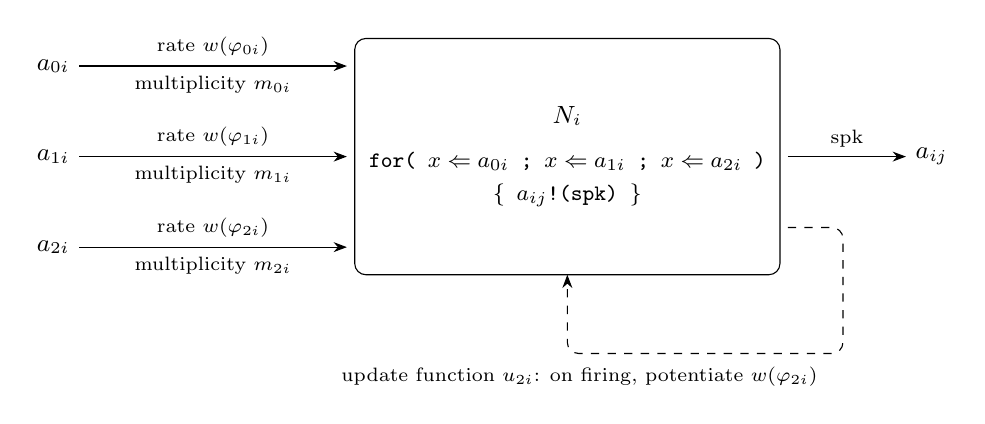
\begin{tikzpicture}[>=Stealth]
  \node[draw, rounded corners, minimum width=54mm, minimum height=30mm, align=center] (N) at (0,0)
    {\small $N_i$\\[4pt]
     \footnotesize\ttfamily for( $x\Leftarrow a_{0i}$ ; $x\Leftarrow a_{1i}$ ; $x\Leftarrow a_{2i}$ )\\
     \footnotesize\ttfamily \{\ $a_{ij}$!(spk)\ \}};
  \foreach \k/\y in {0/1.15, 1/0.0, 2/-1.15} {
    \node[anchor=east] (d\k) at (-6.2,\y) {\small $a_{\k i}$};
    \draw[->] (d\k.east) -- node[above, font=\scriptsize, pos=0.5] {rate $\wmap(\varphi_{\k i})$}
              node[below, font=\scriptsize, pos=0.5] {multiplicity $m_{\k i}$} (-2.8,\y);
  }
  \node[anchor=west] (o) at (4.3,0) {\small $a_{ij}$};
  \draw[->] (2.8,0) -- node[above, font=\scriptsize] {spk} (o.west);
  \draw[->, dashed, rounded corners]
    (2.8,-0.9) -- (3.5,-0.9) -- (3.5,-2.5) -- (0,-2.5) -- (0,-1.5);
  \node[font=\scriptsize, anchor=north east] at (3.3,-2.55)
    {update function $u_{2i}$: on firing, potentiate $\wmap(\varphi_{2i})$};
\end{tikzpicture}
\caption{A neuron. The three factors of Definition~\ref{def:propensity} are visible: the weight map
supplies a rate constant per synapse, the marking supplies multiplicity, and the geometric factor is
$1$. The dashed arrow is the refinement entry's update function, which is where plasticity lives.}
\label{fig:neuron}
\end{figure}

\subsection{The keys, and why they form a partition}

\begin{definition}[Synaptic keys]
\label{def:synkeys}
For each synapse $(j,i)$ put
\[
\varphi_{ji} \;\;\triangleq\;\; \inn(a_{ji})\top \;\sepc\; \out(a_{ji})\top ,
\]
the formula holding of a communication redex on $a_{ji}$, and let
$\Phi_{\textsc{comm}} = \{\varphi_{ji}\} \cup \{\varphi_\bot\}$ with
$\varphi_\bot = L^\sharp \wedge \neg\bigvee_{ji}\varphi_{ji}$.
\end{definition}

\begin{proposition}
\label{prop:rnn-admissible}
$\Phi_{\textsc{comm}}$ is admissible, with $\alpha = 2$.
\end{proposition}

\begin{proof}
Distinct synapses are distinct channels, and a communication redex is on exactly one channel, so
(P1) holds; $\varphi_\bot$ gives (P2) by Remark~\ref{rem:default}. Each key has depth $2$ by
Definition~\ref{def:depth}, and checking $\inn(a)\top \sepc \out(a)\top$ against a term is a bag
lookup, so \ref{req:dec} and \ref{req:loc} hold.
\end{proof}

The weight $\wmap(\varphi_{ji})$ is the efficacy of synapse $(j,i)$. Nothing else in the presentation
mentions it.

\subsection{Threshold is join structure}

\begin{proposition}[McCulloch--Pitts, as an expressivity lemma]
\label{prop:mcp}
The threshold presentation of Definition~\ref{def:neuron} realises the monotone Boolean threshold
function $\mathbf{1}[\,\sum_{j} \mathbf{1}[a_{ji}\text{ populated}] \geq \theta_i\,]$: the neuron has
an enabled redex exactly when at least $\theta_i$ of its dendrites carry a pending spike. It uses
$\binom{k_i}{\theta_i}$ join groups.
\end{proposition}

\begin{proof}
A group $S$ is enabled iff every $a_{si}$ for $s \in S$ carries a spike, since $\&$ requires
simultaneous availability of all its binds; the receipt is enabled iff some group is, since $;$
separates alternatives. Some $\theta_i$-subset is fully populated iff at least $\theta_i$ dendrites
are populated. The count of groups is the count of $\theta_i$-subsets.
\end{proof}

So the historical origin of the neuron model --- McCulloch and Pitts' threshold unit \cite{mcp} ---
is not encoded in a weighted GSLT but \emph{is} a for-comprehension, with the threshold appearing as
the arity of the joins and the alternatives as the group separator. We now state this as an
expressivity lemma and not, as the first version implied, as a practical construction, and the
qualification is not cosmetic. $\binom{k}{\theta}$ groups is unusable at realistic fan-in, so the
scalable presentation is the one at $\theta = 1$, where threshold behaviour is trivial and the join
structure carries no weight. What the lemma establishes is that no apparatus beyond the
for-comprehension is needed to \emph{express} a threshold; what it does not establish is that this is
how one would build a large network.

\begin{remark}[The \texttt{where} clause]
Rholang~1.4's for-comprehension carries a \texttt{where} clause \cite{omnibus}, which collapses the
presentation to a single group at the cost of changing the semantics. The guarded form binds all
$k$ dendrites in one group, waits for \emph{all} of them, and only then applies the filter $\phi$.
That is a coincidence detector with a filter, not a threshold unit. The two
presentations agree at $\theta = k$ and differ elsewhere, and which one a modeller wants is a
modelling question. We use $\theta_i = 1$ below, where both are trivial and the group presentation
has $k_i$ single-bind alternatives.
\end{remark}

\begin{remark}[Coincidence versus rate]
$\theta_i = k_i$ gives a pure coincidence detector: the neuron fires only on simultaneous arrival at
every dendrite. $\theta_i = 1$ gives a pure rate integrator: any arrival can trigger it, and the
weights determine how fast. Real cortical neurons sit between, and so does the presentation, with
$\theta$ as the dial. This is a rare case in which a biological parameter and a syntactic parameter
are the same parameter.
\end{remark}

\subsection{The weighted sum, and where the squashing function went}
\label{sec:squash}

Take $\theta_i = 1$, so $N_i$ has $k_i$ single-bind alternatives, and let the marking assign $m_{ji}$
pending spikes to dendrite $a_{ji}$.

\begin{proposition}[Propensity of a neuron]
\label{prop:neuron-prop}
With $\gfac \equiv 1$ and $\chi \equiv 1$, the total propensity of the redexes belonging to neuron
$i$ is
\[
\prop_i \;=\; \sum_{j} \wmap(\varphi_{ji}) \cdot m_{ji} .
\]
\end{proposition}

\begin{proof}
The receipt is persistent, so exactly one input is available on each $a_{ji}$, and the marking
supplies $m_{ji}$ outputs; by Definition~\ref{def:redex} the number of redexes classified
$\varphi_{ji}$ is $1 \cdot m_{ji}$. Definition~\ref{def:propensity} gives $\wmap(\varphi_{ji})m_{ji}$
per synapse, and the classes are disjoint by Proposition~\ref{prop:rnn-admissible}, so
Proposition~\ref{prop:total} lets them be summed.
\end{proof}

Formally this is the weighted sum $\sum_j w_{ji} m_{ji}$ of the textbook artificial neuron, with the
presynaptic activity $m_{ji}$ read as the marking, and it has not been written into any term; it is
what Definition~\ref{def:propensity} computes. The comparison should nevertheless be made carefully,
because the two quantities are not the same kind of thing. $\prop_i$ is a hazard rate, with units of
inverse time, governing a race between exponential clocks. It is not an affine pre-activation waiting
to be passed through an activation function, and the first version of this note wrote as though it
were. What the next corollary shows is that a saturating nonlinearity nevertheless appears, and
appears without being supplied.

\begin{corollary}[The response saturates and nobody wrote it]
\label{cor:sigmoid}
Hold the marking on $i$'s dendrites fixed over a window $[0,\Delta]$. The probability that neuron $i$
fires at least once in the window is
\[
\Pr[\,\text{$i$ fires}\,] \;=\; 1 - \exp\!\big(-\Delta \textstyle\sum_j \wmap(\varphi_{ji}) m_{ji}\big),
\]
a monotone function of the weighted sum, with slope $\Delta$ at the origin and asymptote $1$.
\end{corollary}

\begin{proof}
Under a marking held fixed on $i$'s dendrites the propensity $\prop_i$ is constant, so firings of $i$
within the window are the events of a homogeneous Poisson process of rate $\prop_i$, by
Theorem~\ref{thm:markov} restricted to the sub-chain along which $m_{\cdot i}$ does not change. The
probability of at least one event in $[0,\Delta]$ is $1 - e^{-\prop_i \Delta}$.
\end{proof}

Two provisos, one standard and one easy to miss.

The standard one is that the marking is not in fact frozen, since other neurons are firing into it.
Corollary~\ref{cor:sigmoid} is a statement about a window short enough that the input has not moved,
which is the usual justification for a rate-coded neuron and the usual approximation.

The one that is easy to miss --- and that the first version's proof did miss, freezing only the other
neurons --- is that $i$'s own firings change the marking. A firing consumes a spike from the dendrite
it fired on, so $\prop_i$ drops and the process is not homogeneous past the first event unless the
marking is externally replenished. The hypothesis must therefore be read as freezing $m_{\cdot i}$
against \emph{all} sources of change, $i$'s own consumption included. That is exactly the
standing-input regime in which a rate code is normally discussed, and it is why the statement is
about the first event rather than about a count.

\begin{remark}[Saturating, not logistic]
\label{rem:not-logistic}
$1 - e^{-\Delta x}$ is an exponential saturation function. It is not the logistic
$\sigma(x) = (1+e^{-x})^{-1}$, and the first version of this note said that it was --- in this
section, and in its abstract, where the emergence of a logistic response was offered as a selling
point. The correct claim is worth as much and should be stated exactly: \emph{a saturating nonlinear
activation emerges from exponential race semantics without being programmed into the term}. No
squashing function was supplied and none is needed. A neuron under enormous drive still cannot fire
more than once per event, so its firing probability per window is bounded by $1$ however large the
weighted sum grows, and that bound is the waiting-time law of the chain rather than a modelling
choice.
\end{remark}

\subsection{Boundedness}
\label{sec:rnn-bounded}

\begin{lemma}[Boundedness]
\label{lem:bounded}
Let $f_i = |\mathrm{post}(i)|$ be the fan-out of neuron $i$. If $f_i \leq \theta_i$ for every $i$,
the total number of pending spikes is non-increasing along every run, the reachable term set is
finite, and $\mathsf{Net}$ is term-finite in the sense of Definition~\ref{def:bounded}.
\end{lemma}

\begin{proof}
Firing $N_i$ consumes $\theta_i$ pending spikes (one per bind in the selected group) and produces
$f_i$. The total marking therefore changes by $f_i - \theta_i \leq 0$. Since the neurons are
persistent and the channel set is fixed, a term reachable from $\mathsf{Net}$ is determined by its
marking, and markings with at most $|M_0|$ tokens over finitely many channels are finite in number.
\end{proof}

The hypothesis is restrictive: it forbids fan-out exceeding threshold, which most networks want. Two
standard repairs, both expressible in the theory:

\begin{enumerate}[leftmargin=2.2em]
\item \emph{Capacity.} Guard the neuron body's sends by a \texttt{where} clause bounding the
occupancy of the target channel \emph{after} the firing by $c$. The marking is then bounded by $c$
per channel and the state space by $c^{|\vec a|}$, restoring term-finiteness unconditionally. This is
a saturating synapse, and it is what a real one does. The post-firing reading is not fussiness: the
obvious alternative, refusing a send when the target is already full, blocks the consumer and
deadlocks the network (\S\ref{sec:built}).
\item \emph{Leak.} Add a base rule $a_{ji}!(\mathrm{spk}) \leadsto \Nil$ with its own key and weight
$\lambda_{\text{leak}}$. This does not restore term-finiteness by itself but makes the marking
positive-recurrent, which is enough for stationary analysis and classical simulation, though it falls
outside the finite-matrix treatment adopted in \S\ref{sec:quantum}.
\end{enumerate}

We take capacity in what follows, since \S\ref{sec:rnn-quantum} needs a finite-dimensional
$\mathcal{H}$.

\begin{remark}[The network is a marked graph]
Under Lemma~\ref{lem:bounded}, $\mathsf{Net}$ is a live, bounded, conservative marked graph in the
Petri-net sense, and the analysis of \cite{knots} applies verbatim: a \emph{period} is a firing
schedule returning the marking to its initial value, and it is the right analogue of a timestep. The
weighted-GSLT layer adds what a marked graph does not have, namely a probability distribution over
which of the enabled transitions fires next and how long it takes.
\end{remark}

\subsection{Plasticity is the update function}
\label{sec:plasticity}

\begin{definition}[Local potentiation entry]
\label{def:hebb}
Equip the communication rule's entry at $\varphi_{ji}$ with
\[
u_{ji}(\wmap) \;=\; \wmap\big[\,\varphi_{ji} \mapsto \min\{\,w_{\max},\ \wmap(\varphi_{ji}) + \eta\,\}\,\big],
\]
for a potentiation increment $\eta > 0$ and ceiling $w_{\max}$. The ceiling is not cosmetic: with a
quantised increment it is what makes the reachable weight-map set finite, which
Remark~\ref{rem:map-finite} requires of \S\ref{sec:rnn-quantum}.
\end{definition}

So the augmented rule reads, in full:
\begin{center}
\begin{minipage}{0.92\textwidth}
\begin{lstlisting}
COMM . |- (PPar {(PForUser rows p), (POutput n q), ...rest})
        ~> (PPar {(subst ...), ...rest})  [1.0] {
      phi(0,1) => (w_01, hebb(0,1)),
      phi(1,1) => (w_11, hebb(1,1)),
      ...
      phi_bot  => (0.0,  id)
   };
ParCong . | S ~> T |- (PPar {S, ...rest}) ~> (PPar {T, ...rest})  [1.0] { snd };
\end{lstlisting}
\end{minipage}
\end{center}

\begin{theorem}[Learning and inference are one relation]
\label{thm:one-relation}
Let $\mathsf{Net}$ be a weighted GSLT as above. The transition relation of
Definition~\ref{def:transition} on $\Cfg = \Terms \times \Wt$ has two marginals: the projection to
$\Terms$ is the network's inference dynamics, and the projection to $\Wt$ is its learning dynamics.
Neither is a separate process. In particular there is no training schedule, no separate learning
clock, and no distinguished learning phase; the learning rate $\eta$ is not a hyperparameter of an
outer loop but a component of the theory, sitting in the same refinement entry as the weight it
modifies.
\end{theorem}

\begin{proof}
Immediate from Definitions~\ref{def:config} and \ref{def:transition}: a single step produces
$(P', \wmap')$ with $P'$ obtained by the rewrite and $\wmap'$ by the fold of the update function.
\end{proof}

This is the claim the example exists to make, and it is exactly what a static-rate calculus cannot
express. In SPiM a rate is fixed at declaration, so a stochastic $\pi$ model of a neural network can
model the firing but not the learning; one must step outside the calculus, adjust the rates, and
re-run. Here the adjustment is a transition of the same system.

\begin{remark}[How Hebbian this is]
\label{rem:hebbian}
Definition~\ref{def:hebb} potentiates $\varphi_{ji}$ when a communication on $a_{ji}$ fires --- that
is, when a presynaptic spike is consumed by an enabled postsynaptic receipt. The event is local and
activity-dependent, and the condition ``pre and post were jointly involved'' is not a correlation
computed by an observer but the firing of a single rewrite, which by construction requires both
parties. That much is the structural content of Hebb's proposal \cite{hebb} and it is the part worth
having: the event which transmits is the event which potentiates, because a communication is one
rewrite.

It is nevertheless less than Hebbian learning as usually meant, and the first version of this note
was too generous in saying that cells which fire together wire together \emph{literally}. Hebbian
plasticity invokes a correlation between pre- and \emph{postsynaptic firing}; successful transmission
into an enabled receipt is not by itself postsynaptic firing, since the receiving neuron may not
reach threshold. What Definition~\ref{def:hebb} gives is a minimal local Hebbian potentiation rule,
and \S\ref{sec:stdp} says what the timing-dependent version costs.
\end{remark}

\subsection{Spike-timing dependence needs a wider update signature}
\label{sec:stdp}

Spike-timing-dependent plasticity makes $\Delta w$ a function of the interval between pre- and
postsynaptic spikes, potentiating for pre-before-post and depressing for the reverse \cite{stdp}.
The ingredients are available --- the simulator of Definition~\ref{def:ssa} produces a timestamp at
every step --- but the update function of Definition~\ref{def:augmented} cannot see them, since its
type is $\Wt \to \Wt$.

\begin{definition}[Extended update]
\label{def:extended-update}
Replace $u_i : \Wt \to \Wt$ by
\[
u_i \;:\; \Wt \times \mathrm{Match} \times \partial\Terms \times \mathbb{R}_{\geq 0} \times \mathcal{S} \longrightarrow \Wt ,
\]
taking additionally the matched substitution $\sigma$, the position $k$ at which the rule fired, the
current simulation time $t$, and a bounded \emph{trace summary} $\mathcal{S}$ --- for STDP, one
eligibility trace per synapse, itself decaying at a rate specified in the theory.
\end{definition}

Theorem~\ref{thm:markov} survives this extension provided $\mathcal{S}$ is finite-dimensional and
updated deterministically, since one simply enlarges the configuration to
$(P, \wmap, \mathcal{S})$; it does \emph{not} survive an update function reading unbounded history,
which would make the process genuinely non-Markovian and put exact simulation out of reach. The
eligibility-trace formulation of STDP is precisely the standard device for staying inside the
bounded case, and it is pleasant that the constraint arrives here from the requirement that the
chain be a chain rather than from computational convenience.

\subsection{Uniformity: one theory for every network}
\label{sec:rnn-uniform}

Definition~\ref{def:synkeys} gives one key per synapse, so a network with $10^4$ synapses has $10^4$
keys and a network that grows needs a new theory. Reflection removes both problems. Following the
construction of \cite{knots}, take the synapse channels to be structured names
\[
a_{ji} \;=\; @[\,*\mathit{net},\, j,\, i\,],
\]
so that a name predicate can recover the endpoints. Then
\[
\varphi_{\mathrm{syn}} \;\triangleq\; \exists j, i.\; \inn(@[*\mathit{net},j,i])\top \;\sepc\; \out(@[*\mathit{net},j,i])\top
\]
is a single key describing the whole \emph{namespace} of synapses of this network, which is
namespace logic doing what it was built for \cite{namespace}. The weight map then has one entry per
network rather than per synapse; per-synapse efficacies are recovered by letting the entry's value be
a function of the recovered indices, which is the standard move of trading a large map for a small
map with structured keys. A greatest fixed point makes ``every neuron reachable from $i$ eventually
fires'' a single formula rather than an $n$-fold conjunction, which is the uniformity $\nu$ buys
\cite[\S3]{classifier}. In an atomic-name calculus none of this is available: the indices would have
to travel as message payloads and the logic could reach them only by observing traffic.

\subsection{The postselected quantum network}
\label{sec:rnn-quantum}

Replace the real efficacies by amplitudes $z_{ji}\in\Cx$. These amplitudes are not converted to
$|z_{ji}|^2$ rates. Each enabled synaptic communication contributes its complex value directly to
the corresponding entry of $T_0$ in Definition~\ref{def:transition-operator}; derivations with the
same successor configuration add before any measurement. The capacity bound is retained, and the
complex update functions are required to range over a finite amplitude alphabet
$\mathcal{Z}\subset\Cx$. The real potentiation update of Definition~\ref{def:hebb} is therefore
replaced, in this instance, by a chosen map $u_{ji}:\mathcal{Z}^N\to\mathcal{Z}^N$ that may change
both modulus and phase.

The example then satisfies Definition~\ref{def:hilbert}: capacity makes the reachable term set
finite, and the finite alphabet makes the reachable map set finite. The complete reachable graph is
assembled once into $T_0$, normalised to the contraction $T$, and dilated by
Theorem~\ref{thm:unitary-dilation}. One synaptic step uses one auxiliary qubit; $n$ coherent steps
use $n$ fresh auxiliaries; and postselecting their all-zero outcome yields $T^n$ by
Theorem~\ref{thm:postselected-power}.

\begin{remark}[Multiplicity becomes interference]
\label{rem:bosonic}
By Remark~\ref{rem:distinct-contracta}, $m$ indistinguishable pending spikes on $a_{ji}$ can give
$m$ derivations with a common contractum. In the complex network their contributions occupy one
matrix element. If they carry the same amplitude and geometric factor, that element is multiplied by
$m$ and its contribution to a measured probability is proportional to $m^2$; if different
refinement classes contribute opposite phases, it can instead be suppressed or cancelled. This is
not a claimed classical rate law. It is the direct consequence of treating the weights as amplitudes
before measurement, and it is exactly the behaviour the former magnitude-square construction
removed.

Structural congruence does not supply an additional coherent channel. Configurations whose terms are
$\equiv$-equal are one basis state, so there is no Hamiltonian mixing alternative representatives.
All coherence in this example is already visible in the sums defining $T_0$.
\end{remark}

The projectors of Proposition~\ref{prop:projective} remain available. For example,
$\Pi_{\varphi_{\mathrm{syn}}}$ measures whether a postselected configuration has an available
synaptic transmission. After $n$ successful steps its expectation is given by the conditional formula
of \S\ref{sec:quantum-logic}.

\subsection{What this example does not show}

Honesty about scope. The learning here is local and Hebbian; nothing above implements
backpropagation, which needs a global error signal propagated against the direction of inference.
One can encode such a signal as traffic on a second family of channels with its own keys, and the
apparatus does not forbid it, but the result would no longer have the property that makes
Theorem~\ref{thm:one-relation} interesting --- the error channel is an outer loop wearing a costume.
Whether a genuinely local weighted-GSLT learning rule can match backpropagation is not a question
this note answers, and the honest statement is that the example demonstrates a \emph{mechanism} for
plasticity inside the calculus, not a competitive learning algorithm.

Nor do we claim biological fidelity. The neuron of Definition~\ref{def:neuron} has no membrane
potential, no refractory period, and no dendritic geometry. The first two are easy additions --- a
potential is a payload, a refractory period is a guard --- and the third is what the geometric factor
$\gfac$ of \S\ref{sec:geometric} is for, which is a use we have not developed.

\section{Implementation}
\label{sec:impl}

\subsection{Surface syntax}
\label{sec:surface}

The weighting is a decoration of MeTTaIL's \texttt{rewrites} block, and it should read as one. The
existing surface is
\begin{center}
\begin{minipage}{0.88\textwidth}
\begin{lstlisting}
rewrites {
    Exec    . |- (PDrop (NQuote P)) ~> P;
    ParCong . | S ~> T |- (PPar {S, ...rest}) ~> (PPar {T, ...rest});
}
\end{lstlisting}
\end{minipage}
\end{center}
and the weighted surface adds a bracketed weight and a brace block after the rule, in both cases
optional:
\begin{center}
\begin{minipage}{0.88\textwidth}
\begin{lstlisting}
rewrites {
    // base rule: [scalar] { key => (weight, update) }
    COMM . |- (PPar {(PForUser rows p), (POutput n q), ...rest})
            ~> (PPar {(subst rows p q), ...rest})   [1.0] {
        in(n)TOP | out(n)@fast  => (2.5, scale(0.9)),
        in(n)TOP | out(n)TOP    => (0.7, id),
        default                 => (0.0, id)
    };

    // base rule, unweighted: defaults to [1.0] { default => (1.0, id) }
    Exec . |- (PDrop (NQuote P)) ~> P;

    // context rule: [geometric factor] { fold }
    ParCong . | S ~> T |- (PPar {S, ...rest}) ~> (PPar {T, ...rest})  [1.0] { snd };
}
\end{lstlisting}
\end{minipage}
\end{center}

Notes on the design. \texttt{default} is sugar for the completion of
Remark~\ref{rem:default} --- the elaborator synthesises
$L^\sharp \wedge \neg\bigvee_i \varphi_i$ --- so a modeller writes exclusive keys and gets a
partition. Exclusivity itself is checked at elaboration time and is a hard error, not a warning,
since Proposition~\ref{prop:classify} fails without it. Keys are written in the concrete syntax of
the generated logic; the two shown are ordered from more to less specific purely for readability,
since exclusivity means order is semantically irrelevant. A context rule's default factor is
$1$ and its default fold is \texttt{snd}, which together implement ``addressing is free and does not
touch the map'' (\S\ref{sec:geometric}).

\subsection{What is built}
\label{sec:built}

The first version of this note measured itself against a prototype called \texttt{mettail-gillespie},
whose \texttt{TermRef} was an opaque identifier, whose spatial behaviours were a hand-rolled enum,
whose rates were clamped to the unit interval, and whose quantum module was amplitude bookkeeping
over a classical branching structure. That crate no longer exists. It has been superseded by
\texttt{rho-weighted} \cite{gillespie-crate}. The classical simulator and exhaustive graph builder are
the implementation basis used below. The unitary-dilation construction of \S\ref{sec:quantum} is a
new specification target: the old amplitude bookkeeping and the former density-operator path do not
constitute an implementation of it.

\paragraph{What the crate is.} A \emph{simulator}, and deliberately not the interpreter. The
interpreter maintains the state of a running shard; the simulator answers what would happen if,
across a family of hypothetical configurations, and yields transition graphs, generators and
parameter sweeps rather than a single history. That separation is what makes exhaustive graph
construction, greatest fixed points and the finite matrix construction required by
\S\ref{sec:quantum} affordable here and unaffordable there, and it is why the crate owns its own space --- an immutable channel index with
cheap forking --- rather than a tuple space with checkpoints. It shares the interpreter's matching
semantics without sharing its code paths, which makes agreement between them an obligation rather
than a theorem; see below.

\paragraph{Correspondence with this note.}
\begin{center}
\begin{tabular}{@{}>{\raggedright\arraybackslash}p{0.38\textwidth}>{\raggedright\arraybackslash}p{0.56\textwidth}@{}}
\toprule
Specification & Implementation \\
\midrule
Definitions \ref{def:partition}--\ref{def:reqs}, admissibility & partition and fragment checks; failure is an error, never a fallback \\
Proposition~\ref{prop:classify}, classification & the classifier, total by construction \\
Definition~\ref{def:propensity}, propensity & organised by redex, per Proposition~\ref{prop:total} \\
Definition~\ref{def:ssa}, the SSA & the sampler, with provenance recorded per run \\
Theorem~\ref{thm:markov}, the generator & exhaustive graph plus $Q$, diagonal per Remark~\ref{rem:selfloop} \\
Definition~\ref{def:extended-update}, updates & the update context: bindings, position, clock, trace \\
\S\ref{sec:rnn}, the network & the worked example, end to end \\
Definitions \ref{def:transition-operator}--\ref{def:iterated-dilation}, the quantum path & outstanding: sparse $T_0$, global normalisation, defects, dilation \\
\bottomrule
\end{tabular}
\end{center}

\paragraph{Three constraints an implementation exposed.} These are the reason this section is worth
reading rather than a table of ticks.

\begin{enumerate}[leftmargin=2.2em]
\item \emph{Multiplicity is invisible in a trace.} The superseded prototype omitted the cardinality
of $K(r,\varphi,P)$ entirely, and its traces looked entirely plausible; nothing an eye could catch
distinguishes a chain running at the wrong rate from one running at the right rate. Acceptance
therefore has to be statistical rather than observational. The birth--death theory is checked against
a truncated Poisson law, with a control asserting that the Poisson and geometric laws are half a unit
of total variation apart, so that the test cannot pass vacuously against a chain that ignores
multiplicity.
\item \emph{A capacity guard must be evaluated post-firing.} The obvious reading of the guard of
\S\ref{sec:rnn-bounded} --- refuse a send when the target channel is already at capacity --- blocks
the consumer and deadlocks the network. The guard must bound occupancy \emph{after} the firing it
gates. Relatedly, a hard capacity makes a token amplifier absorbing rather than live, which is a stop
and not a deadlock; a network that is to saturate and keep running wants the leak rule of
\S\ref{sec:rnn-bounded} instead, trading term-finiteness for positive recurrence and thereby giving
up \S\ref{sec:quantum}.
\item \emph{Contractivity is global.} Entrywise bounds on complex weights do not bound the norm of
the assembled transition operator, because amplitudes can add within a column and within a target
entry. A quantum backend must build or bound $\|T_0\|$ first, then construct $T$, $D_T$, and
$D_{T^\dagger}$; dilating each weight independently implements a different map.
\end{enumerate}

\paragraph{What is outstanding.} Four items follow.
\begin{enumerate}[leftmargin=2.2em]
\item \emph{The logic is hand-written, not generated.} The connectives of \S\ref{sec:logic} are
implemented by hand behind a port whose interface is the one an OSLF-generated instance would
implement, so the swap is at the boundary rather than through the simulator, which was the design
intent. Until it lands, the genericity over GSLTs claimed in \S\ref{sec:intro} is argued and not
demonstrated, and that is the largest gap in the note.
\item \emph{Surface syntax.} \S\ref{sec:surface} is a design and not a grammar. It needs parser and
tree-sitter changes in a separate repository on a separate release cadence; theories are built
programmatically today, and nothing else in the crate depends on the syntax landing.
\item \emph{Faithfulness.} Because the simulator and the interpreter share semantics but not code
paths, their agreement is a permanent obligation. What runs today is a differential against an
independently written reference matcher over a corpus of several hundred cases, together with a
negative control establishing that the corpus can detect a broken matcher. The differential against
the interpreter's own matcher is written, is gated behind a build feature, and has not been run,
because the workspace it needs does not currently build from a clean checkout. The gap is visible in
the test output by design rather than recorded only here.
\item \emph{The dilation backend.} The crate does not yet assemble the sparse complex matrix $T_0$,
compute a certified normalisation, form the defect square roots, or synthesize the auxiliary-qubit
unitary. Until those pieces exist, \S\ref{sec:quantum} is a mathematical construction rather than an
implemented execution path.
\end{enumerate}

\paragraph{Two known incompletenesses.} First, the partition check evaluates (P1) and (P2) against a
supplied set of witnesses. It is therefore a sound \emph{refuter} --- an overlap it reports is real
--- and not a proof of admissibility, which would require deciding entailment in the generated logic.
By Observation~\ref{obs:closure} this is exactly the price of taking the external branch, and it
should be read as such rather than as a deficiency of the check. Second, the checkable-fragment gate
currently admits modal and fixed-point formulae as keys, which \ref{req:str} forbids; enforcing
\ref{req:str} at elaboration time is a small change and is the precondition for the incremental
scheme below.

\subsection{Incremental propensity}
\label{sec:incremental}

Lemma~\ref{lem:locality} licenses the standard optimisation. Maintain $\prop$ as a Fenwick tree over
$(r,\varphi)$ classes with per-class redex lists; after firing at position $k$, reclassify only
redexes within radius $\alpha + |L| + |R|$ of $k$, and additionally rescale the classes whose weight
the update function touched --- which for Definition~\ref{def:hebb} is exactly one class. The second
part is the only respect in which dynamic weight maps cost anything at run time, and it is cheap
precisely when update functions are sparse. A modeller who writes an update function touching every
entry pays a full recomputation of $\prop_0$ per step, and should be told so.

\section{Weights and costs}
\label{sec:cost}

Cost accounting and weighting both decorate rewrites, and it is worth stating plainly that they are
different decorations doing different jobs.

A cost decoration attaches to a rewrite a debit against a token stack, and the funding judgment
$\Sigma \funds \Delta$ --- decidable, total, monotone in supply --- decides whether a step may occur
at all \cite{costmonad}. It is implemented in the transpiler branch as
\texttt{OslfResourceLogic}, with a supply multiset keyed by signature and a demand list, one token
per signed term, and conformance laws asserting soundness, rejection of underfunding, supply
monotonicity, and decidability. A weight decoration attaches a rate, and decides how fast and how
often. The composition is one-directional:

\begin{definition}[Funding gate]
\label{def:gate}
For a redex $(k,\sigma)$ of rule $r$, let $\Delta(r,k,\sigma)$ be the demand it incurs and
$\Sigma(P,k)$ the supply available at that location. Put
$\chi(r,k,\sigma) = 1$ if $\Sigma(P,k) \funds \Delta(r,k,\sigma)$ and $0$ otherwise.
\end{definition}

\begin{proposition}[Cost gates the support, weight distributes over it]
\label{prop:gate}
With $\chi$ as in Definition~\ref{def:gate}, the coalgebra of Definition~\ref{def:coalgebra}
restricts to the funded sub-transition-system: unfunded redexes have propensity zero and contribute
nothing to $\prop_0$, while among funded redexes the distribution is unchanged from the
cost-free case up to normalisation.
\end{proposition}

\begin{proof}
$\chi$ appears as a multiplicative factor in Definition~\ref{def:propensity}, taking values in
$\{0,1\}$; a zero factor removes the term from the sum, and the remaining terms are untouched.
\end{proof}

Three consequences worth recording.

\emph{The gate is decidable, so the simulator stays exact.} If funding were a real-valued penalty
rather than a Boolean, the propensity would depend on an optimisation and the chain would no longer
be simulable by Definition~\ref{def:ssa}. The decidability law of the resource logic is doing real
work here.

\emph{Exhaustion is a halting condition, not a deadlock.} $\prop_0 = 0$ when every enabled redex is
unfunded, and Definition~\ref{def:ssa} halts. The chain has reached an absorbing state, which is the
correct reading: a system that cannot pay for any of its available transitions has stopped, and the
waiting time to the next event is infinite rather than undefined.

\emph{The neural example acquires a metabolism.} Give the communication rule a phlogiston demand per
firing and the network of \S\ref{sec:rnn} has an energy budget: a neuron whose local supply is
exhausted has propensity zero regardless of its synaptic weights, and the network's activity is
bounded by its funding rather than by its capacity guard. Weight is what a synapse is worth; cost is
what a spike costs. Separating them is what lets a model say that a strong synapse on a starving
neuron is silent, which is a statement neither decoration makes alone. This is the point of contact
with the mortal-computation reading of \cite{scientist}, and we go no further with it here.

\section{Open threads}
\label{sec:open}

\begin{enumerate}[leftmargin=2.2em]
\item \emph{A combined logic.} \S\ref{sec:quantum-logic} supplies projectors for states conditioned on
an all-zero auxiliary record. What one wants is a temporal logic that can speak both about generated
configuration predicates and about success and failure histories, for example a modality for ``after
$n$ successful applications of $T$''. The conditioning event must be part of the semantics rather
than silently renormalised away.
\item \emph{Weighted bisimulation.} The category \textbf{GSLT} has bisimulation-preserving maps as
morphisms \cite{omnibus}. Rate bisimulation is the natural real-valued candidate. In the complex case
a relation must preserve the amplitude operator, not merely the measured populations: a plausible
criterion is an intertwiner for $T$, but it is not yet clear whether the defect operators, or only the
postselected completely positive map $\rho\mapsto T\rho T^\dagger$, must also be preserved.
\item \emph{Derivation-sensitive phases.} Definition~\ref{def:transition-operator} sums over
individual derivations, but all derivations in one refinement class read the same map entry. More
fine-grained interference requires keys or decorations that distinguish derivations without making
the map grow with the term. Whether that can be reconciled with Lemma~\ref{lem:locality} is open.
\item \emph{Efficient dilation.} The canonical defect square roots are mathematically explicit and can
be dense even when $T_0$ is sparse. A practical backend should exploit sparse block encodings,
approximate polynomial square roots, or a larger but cheaper dilation while preserving the exact
all-zero block. The resource trade-off between auxiliary dimension, circuit depth, and postselection
probability has not been developed here.
\item \emph{Geometric factors.} \S\ref{sec:geometric} introduces $\gfac$ as a real structural
weight. Definition~\ref{def:transition-operator} treats it as an amplitude multiplier. A modeller who
wants $|T_{\mathfrak{c}',\mathfrak{c}}|^2$ to retain a particular classical geometric scaling may
instead want $\sqrt{\gfac}$. The right choice is part of the quantum model and should not be hidden
behind a supposed conservativity theorem.
\item \emph{Quantale weights.} A quantale-valued codomain gives a fuzzy calculus, and \cite{fuzzy}
develops the flat-substitution instance independently. The criterion is no longer the existence of a
map into $\Rnn$: the real and complex cases already have different operational readings. The open
question is instead which algebraic structure turns a weighted coalgebra into an executable object
and what replaces unitary dilation outside $\Cx$.
\item \emph{Infinite configuration spaces.} Remark~\ref{rem:map-finite} uses finiteness to make
$T_0$ and its defects concrete. The construction extends to bounded contractions on a separable
Hilbert space, but reachable complex weight maps can easily make the operator unbounded or its norm
noncomputable. Useful syntactic conditions guaranteeing boundedness would remove the present
quantisation requirement.
\item \emph{Modal-key locality.} \ref{req:str} excludes behavioural modalities from keys because
Lemma~\ref{lem:locality} fails for them, and a weight that depends on what a redex can do next is a
natural thing for a modeller to want. The question is whether a bounded-lookahead modality
$\langle K\rangle^{\le n}$ admits a locality lemma with radius depending on $n$, or whether modal
keys simply cost global reclassification at every step.
\end{enumerate}

\begin{thebibliography}{99}

\bibitem{classifier} L.\ G.\ Meredith. \emph{Classifying knots with spatial--behavioural logics.}
F1R3FLY.io working note, 2026.

\bibitem{costmonad} L.\ G.\ Meredith. \emph{Cost accounting as an endofunctor on continued
interactive GSLTs.} F1R3FLY.io working note, 2026.

\bibitem{costspacetime} L.\ G.\ Meredith. \emph{Cost, spacetime, and the geometry/matter split on
reduction graphs.} F1R3FLY.io working notes, 2026.

\bibitem{fuzzy} \emph{Fuzzy rho-calculus: a quantale-graded interaction, and its lift to ciGSLTs with
binding.} F1R3FLY.io working note, 2026.

\bibitem{gibson-bruck} M.\ A.\ Gibson and J.\ Bruck. Efficient exact stochastic simulation of
chemical systems with many species and many channels. \emph{Journal of Physical Chemistry A}
104(9):1876--1889, 2000.

\bibitem{gillespie77} D.\ T.\ Gillespie. Exact stochastic simulation of coupled chemical reactions.
\emph{Journal of Physical Chemistry} 81(25):2340--2361, 1977.

\bibitem{gillespie-crate} F1R3FLY.io. \texttt{mettail-gillespie}: stochastic and quantum Gillespie
simulation extensions for MeTTaIL rewrite rules. \texttt{F1R3FLY-io/publications},
\texttt{rho-life/Gillespie}, 2026.

\bibitem{hebb} D.\ O.\ Hebb. \emph{The Organization of Behavior.} Wiley, 1949.

\bibitem{knots} L.\ G.\ Meredith. \emph{Knots as cost-accounted processes.} F1R3FLY.io working note,
2026.

\bibitem{mcp} W.\ S.\ McCulloch and W.\ Pitts. A logical calculus of the ideas immanent in nervous
activity. \emph{Bulletin of Mathematical Biophysics} 5:115--133, 1943.

\bibitem{mettacalc} L.\ G.\ Meredith et al. \emph{The MeTTa calculus.} F1R3FLY.io, 2026.

\bibitem{mettail} F1R3FLY.io. \texttt{mettail-rust}: the \texttt{language!} macro and its shipped
language definitions. \texttt{F1R3FLY-io/mettail-rust}, 2026.

\bibitem{namespace} L.\ G.\ Meredith and M.\ Radestock. Namespace logic: a logic for a reflective
higher-order calculus. In \emph{Trustworthy Global Computing}, LNCS 3705, Springer, 2005.

\bibitem{omnibus} L.\ G.\ Meredith. \emph{Graph-Structured Lambda Theories: A Reference for the
Working Developer.} F1R3FLY.io, 2026.

\bibitem{priami} C.\ Priami. Stochastic $\pi$-calculus. \emph{The Computer Journal} 38(7):578--589,
1995.

\bibitem{scientist} L.\ G.\ Meredith. \emph{The Mortal Scientist.} F1R3FLY.io working note, 2026.

\bibitem{spim} A.\ Phillips and L.\ Cardelli. A correct abstract machine for the stochastic
pi-calculus. In \emph{Bioconcur}, 2004.

\bibitem{spim-sim} A.\ Phillips and L.\ Cardelli. Efficient, correct simulation of biological
processes in the stochastic pi-calculus. In \emph{Computational Methods in Systems Biology}, LNCS
4695, Springer, 2007.

\bibitem{stdp} G.\ Q.\ Bi and M.\ M.\ Poo. Synaptic modifications in cultured hippocampal neurons:
dependence on spike timing, synaptic strength, and postsynaptic cell type. \emph{Journal of
Neuroscience} 18(24):10464--10472, 1998.

\end{thebibliography}

\end{document}
